%% Preamble %%
\documentclass[paper=a4]{article}

\usepackage{float}
\usepackage{geometry}
\geometry{verbose,tmargin=2.25cm,bmargin=2cm,lmargin=2.25cm,rmargin=2cm}
\geometry{a4paper}
\usepackage{multirow}


\usepackage[T1]{fontenc}
\usepackage{fourier}
\usepackage[utf8]{inputenc}
\usepackage[spanish]{babel}				

\usepackage{amsmath,amsfonts,amsthm} % Math packages
\usepackage[pdftex]{graphicx}	

\makeatletter
%%%%%%%%%%%%%%%%%%%%%%%%%%%%%% User specified LaTeX commands.
\usepackage{fancyhdr}
\usepackage{lscape}
\pagestyle{fancy}
\lhead{Electr\'onica II 22.12}
\chead{TPL1}
\rhead{ITBA}
\renewcommand{\headrulewidth}{1pt}
\renewcommand{\footrulewidth}{1pt}

\makeatother

\usepackage{babel}
\addto\shorthandsspanish{\spanishdeactivate{~<>}}

\begin{document}

\tableofcontents
\newpage

\section{Objetivos - Par\'ametros del dise\~no}

En el presente trabajo de laboratorio se realiza el diseño y an\'alisis b\'asico del funcionamiento de una fuente regulada de tensi\'on, que cumple con las siguientes especificaciones:

\begin{center}
\begin{tabular}{|c|c|}
\hline 
Rango de tension de salida & $IO_{MAX}$\\
\hline 
\hline 
$4V \leq V_O \leq 10V$ & $1.5A$\\
\hline 
\end{tabular}
\end{center}

El diseño se implementar\'a en un PCB siguiendo determinadas consideraciones, y se realizar\'a otro PCB adicional como banco de pruebas.

\section{Dise\~no del sistema}

Para implementar el dise\~no en cuesti\'on, se propone un circuito de regulaci\'on serie, el cual puede modelarse con el siguiente esquema.

\begin{figure}[!ht]
\begin{centering}
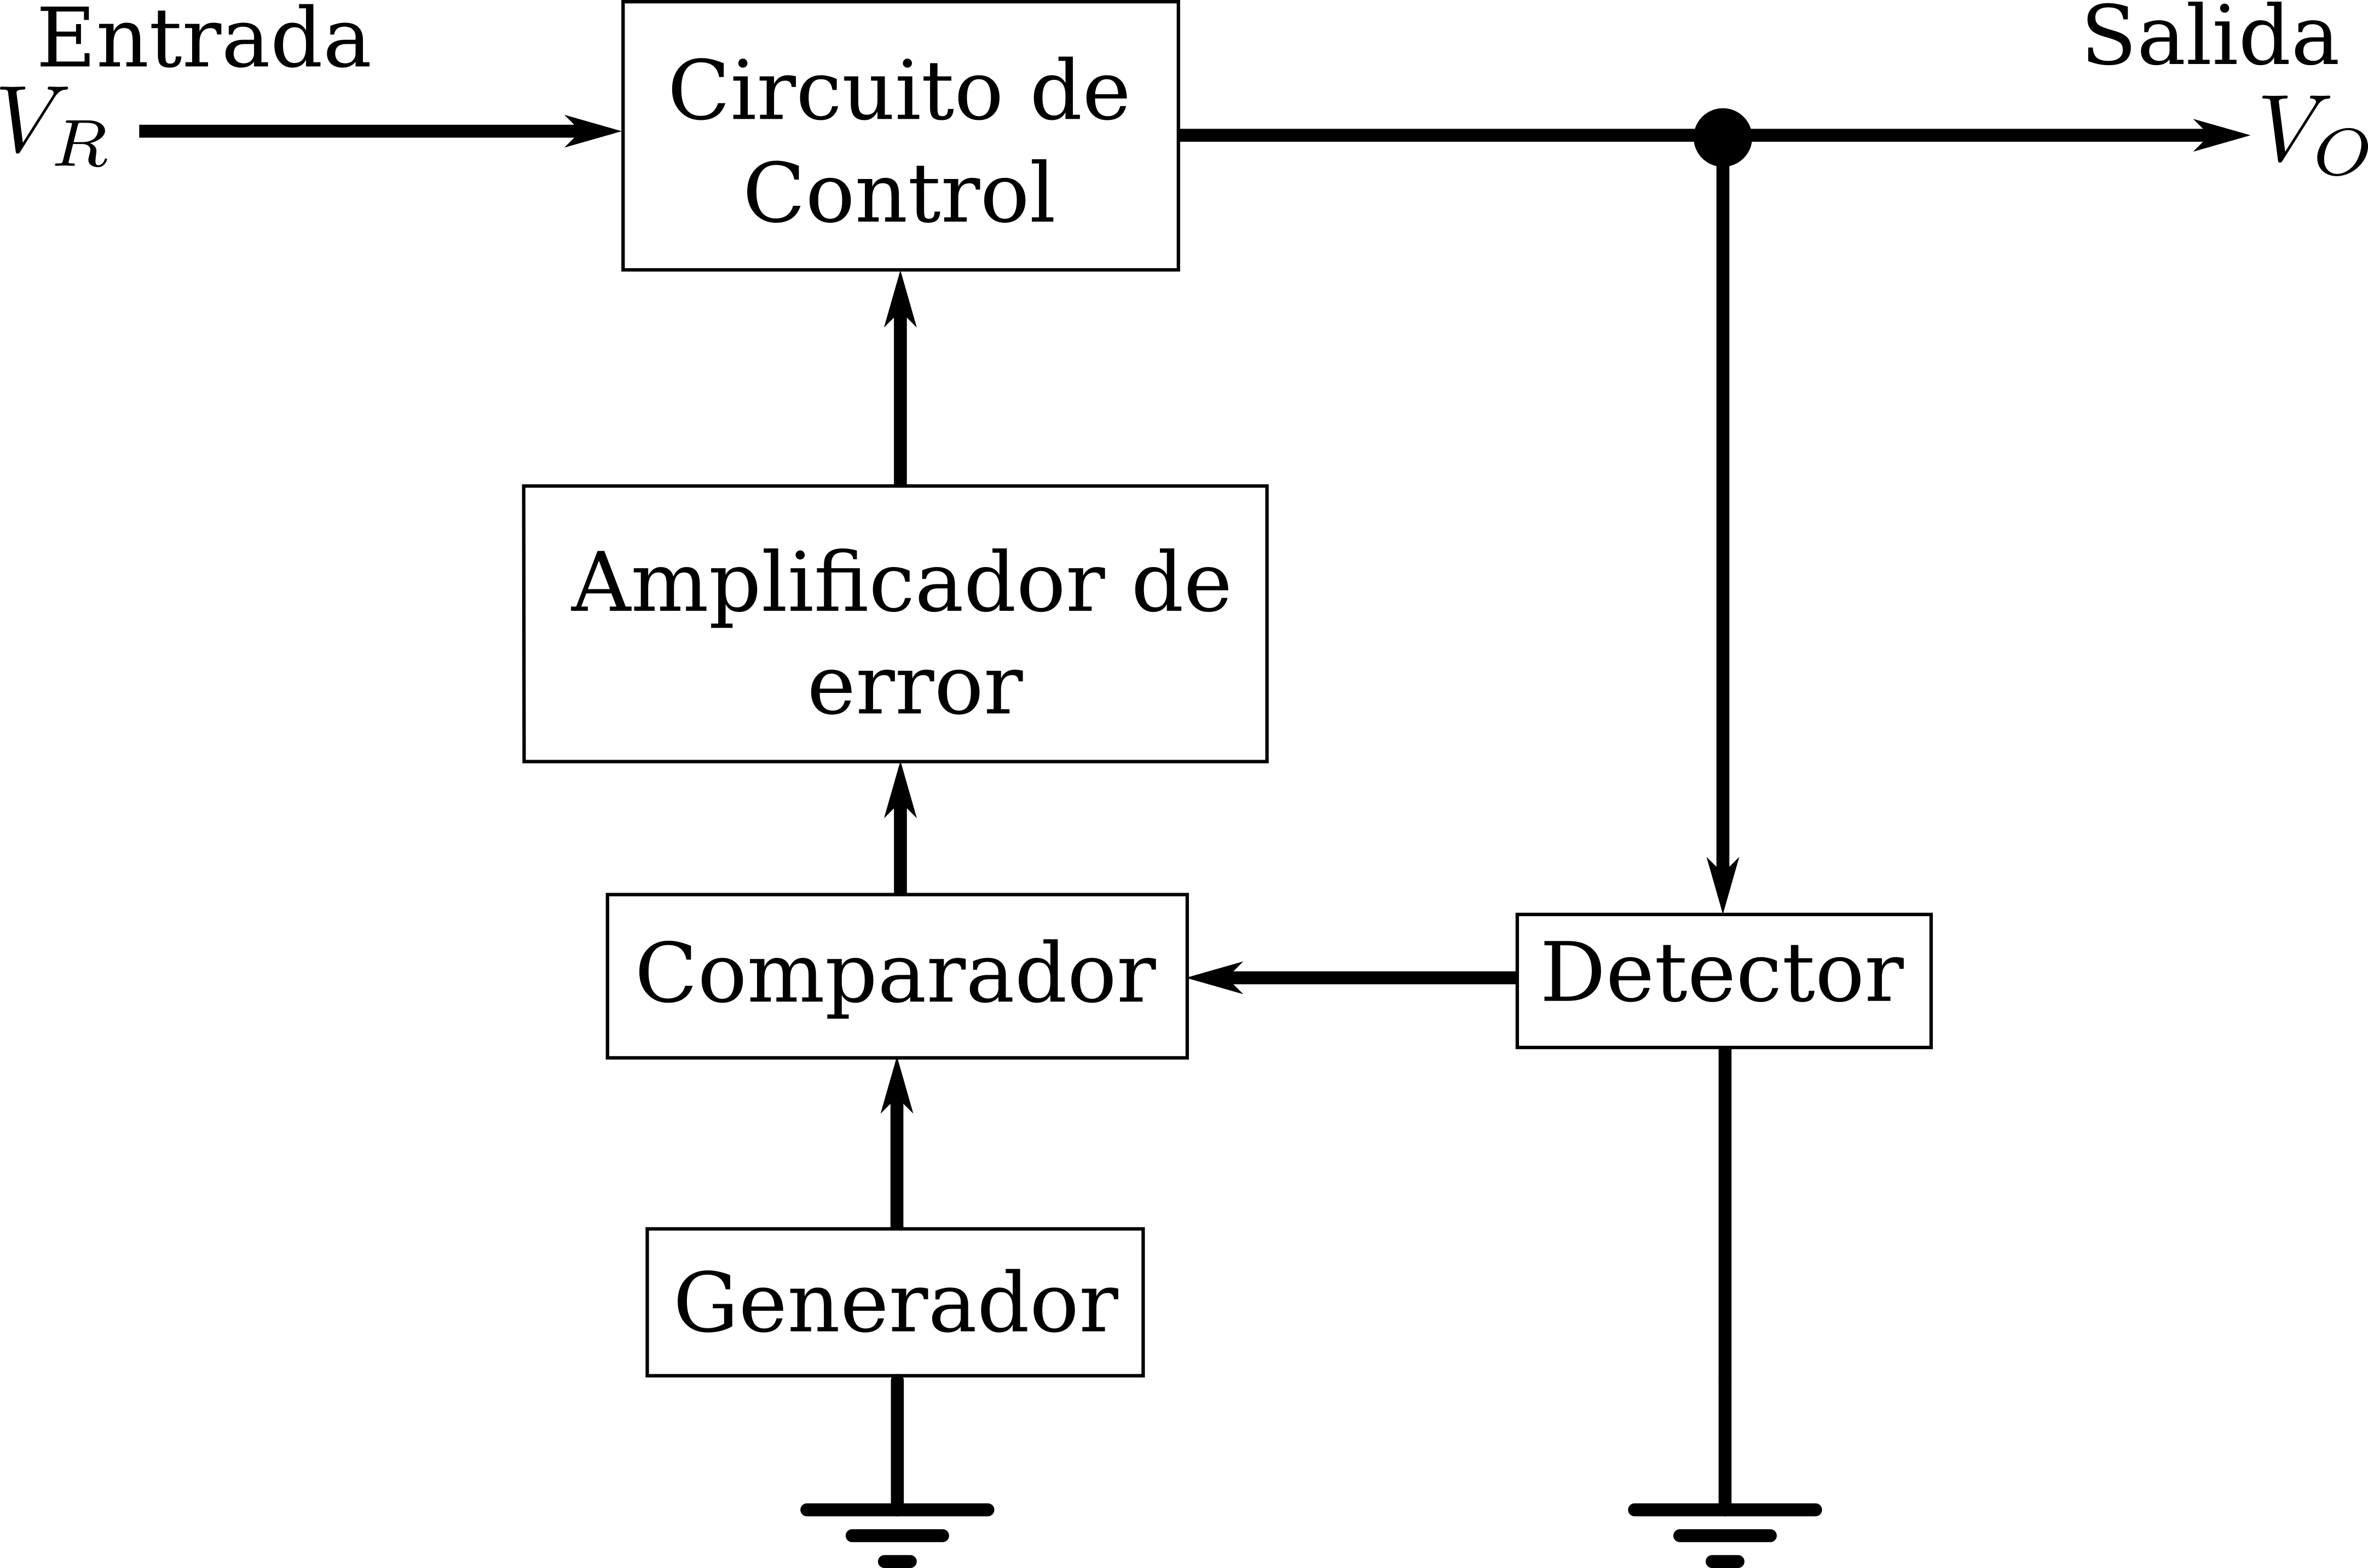
\includegraphics[scale=0.35]{Imagenes/bloquesSerie.png}
\par\end{centering}
\caption{Diagrama en bloques de un regulador serie}

\end{figure}

La caracter\'istica de 'serie' refiere a que el elemento de control se encuentra en serie a la carga $R_L$. En base a dicho esquema, se propone el siguiente circuito.

\begin{figure}[!ht]
\begin{centering}
\includegraphics[scale=0.32]{Imagenes/CircuitoSinCap.png}
\par\end{centering}
\caption{Circuito regulador serie propuesto}

\end{figure}

La caracter\'istica de regulaci\'on se basa en un lazo de realimentaci\'on negativa entre la salida, el detector, el amplificador de error y el circuito de control. Si se supone que por un momento el valor de $V_O$ aumenta, en consecuencia el valor a la salida del detector tambi\'en aumenta. Dado que la tensi\'on provista por el generador es constante, la diferencia entre la tensi\'on a la salida del detector y el generador aumentar\'a, por lo que la tensi\'on a la salida del operacional tambi\'en. Al ocurrir esto, el transistor $T_1$ conducir\'a m\'as corriente entre colector y emisor. Dado que la corriente provista por el pre-regulador con $T_3$ es constante (como se tratar\'a posteriormente), lo que sucede entonces es que se le quita corriente a la base del transistor $T_2$. En consecuencia, \'este conduce menos corriente, por lo que la carga $R_L$ recibe menos corriente, reestableciendo el valor de $V_O$.\par
Cada bloque por separado se trata en las subsecciones siguientes.

\subsection{Circuito de control}

\begin{figure}[!ht]
\begin{centering}
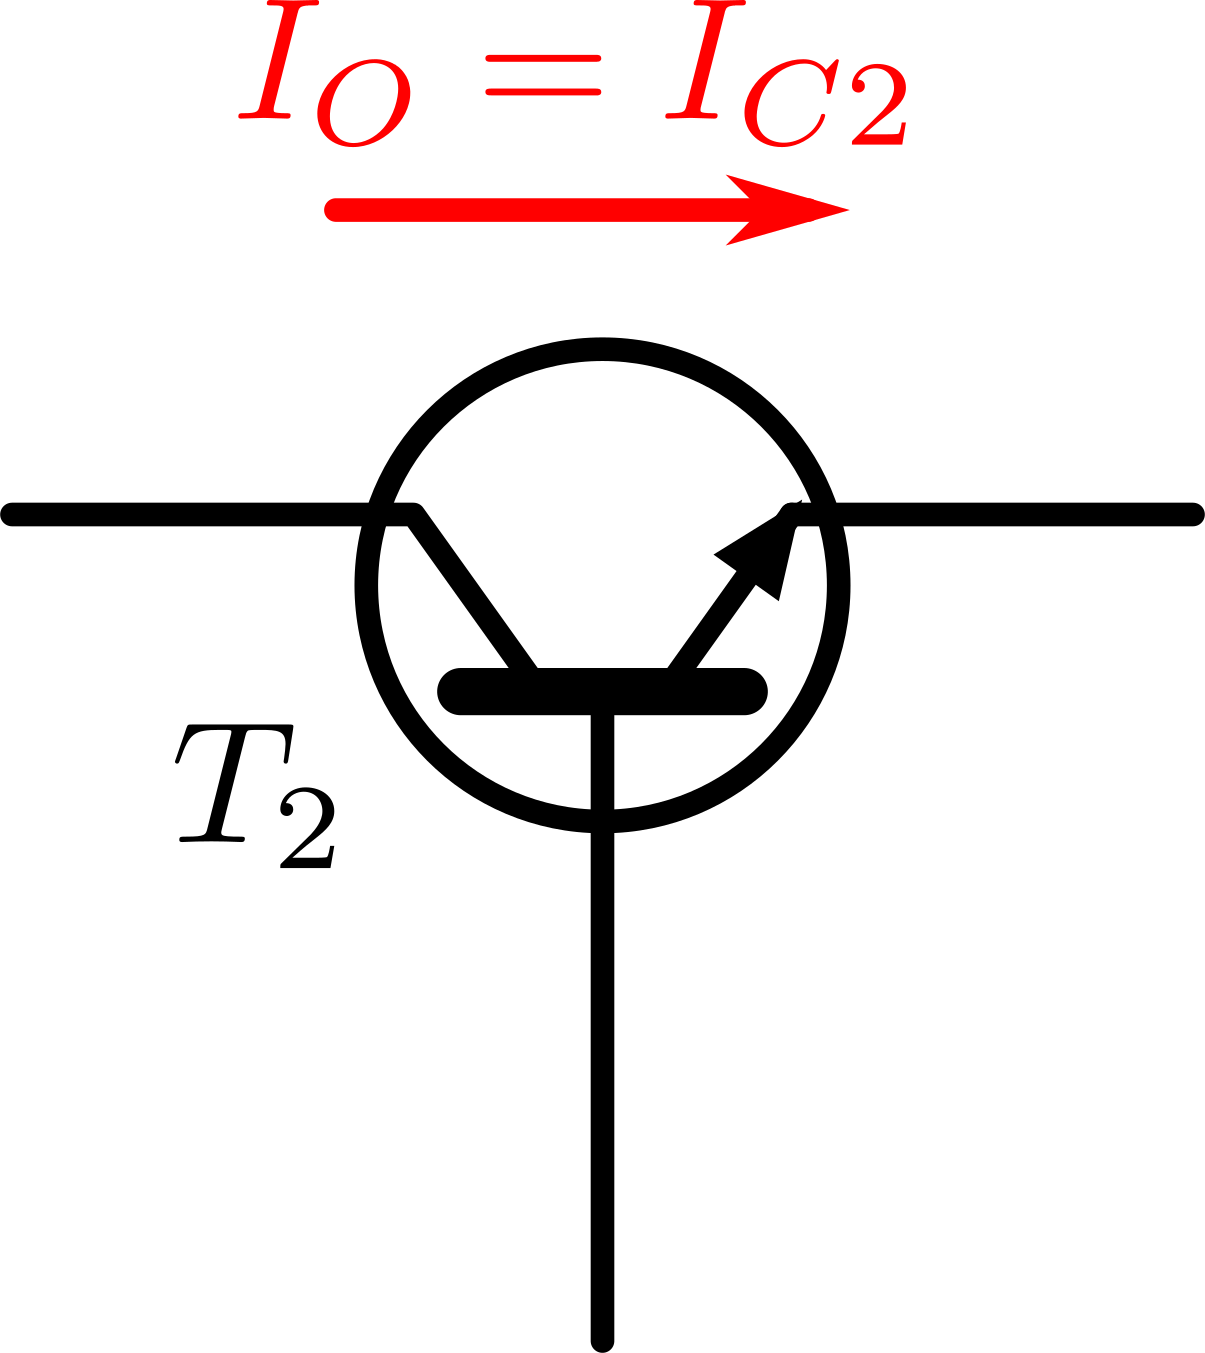
\includegraphics[scale=0.5]{Imagenes/Control.png}
\par\end{centering}
\caption{Circuito de control}

\end{figure}

El circuito de control, en este caso "serie", regula la intensidad de corriente que circula hacia la carga $R_L$ (a trav\'es de los otros bloques) de acuerdo al valor de dicha carga. El control es realizado de manera tal que el valor de $V_O$ seteado se mantenga, como se explic\'o anteriormente.
Sabiendo que la $I_O$ m\'axima en regulaci\'on es de $1.5A$, se elije un transistor adecuado que en primera instancia pueda conducir dicha corriente, y luego verificar que la potencia m\'axima que vaya a disipar est\'e dentro de la dada por el fabricante.\par
Para dar un cierto margen a la corriente y poder alcanzar el valor de $I_O$ m\'axima sin problemas se elije $T_2 = TIP112$, cuya m\'axima corriente de emisor es de $2A$.
En la secci\'on de c\'alculo de disipador se detalla el an\'alisis de la potencia a disipar y la elecci\'on del disipador en caso de necesitarlo.

\subsection{Pre-regulador}

\begin{figure}[!ht]
\begin{centering}
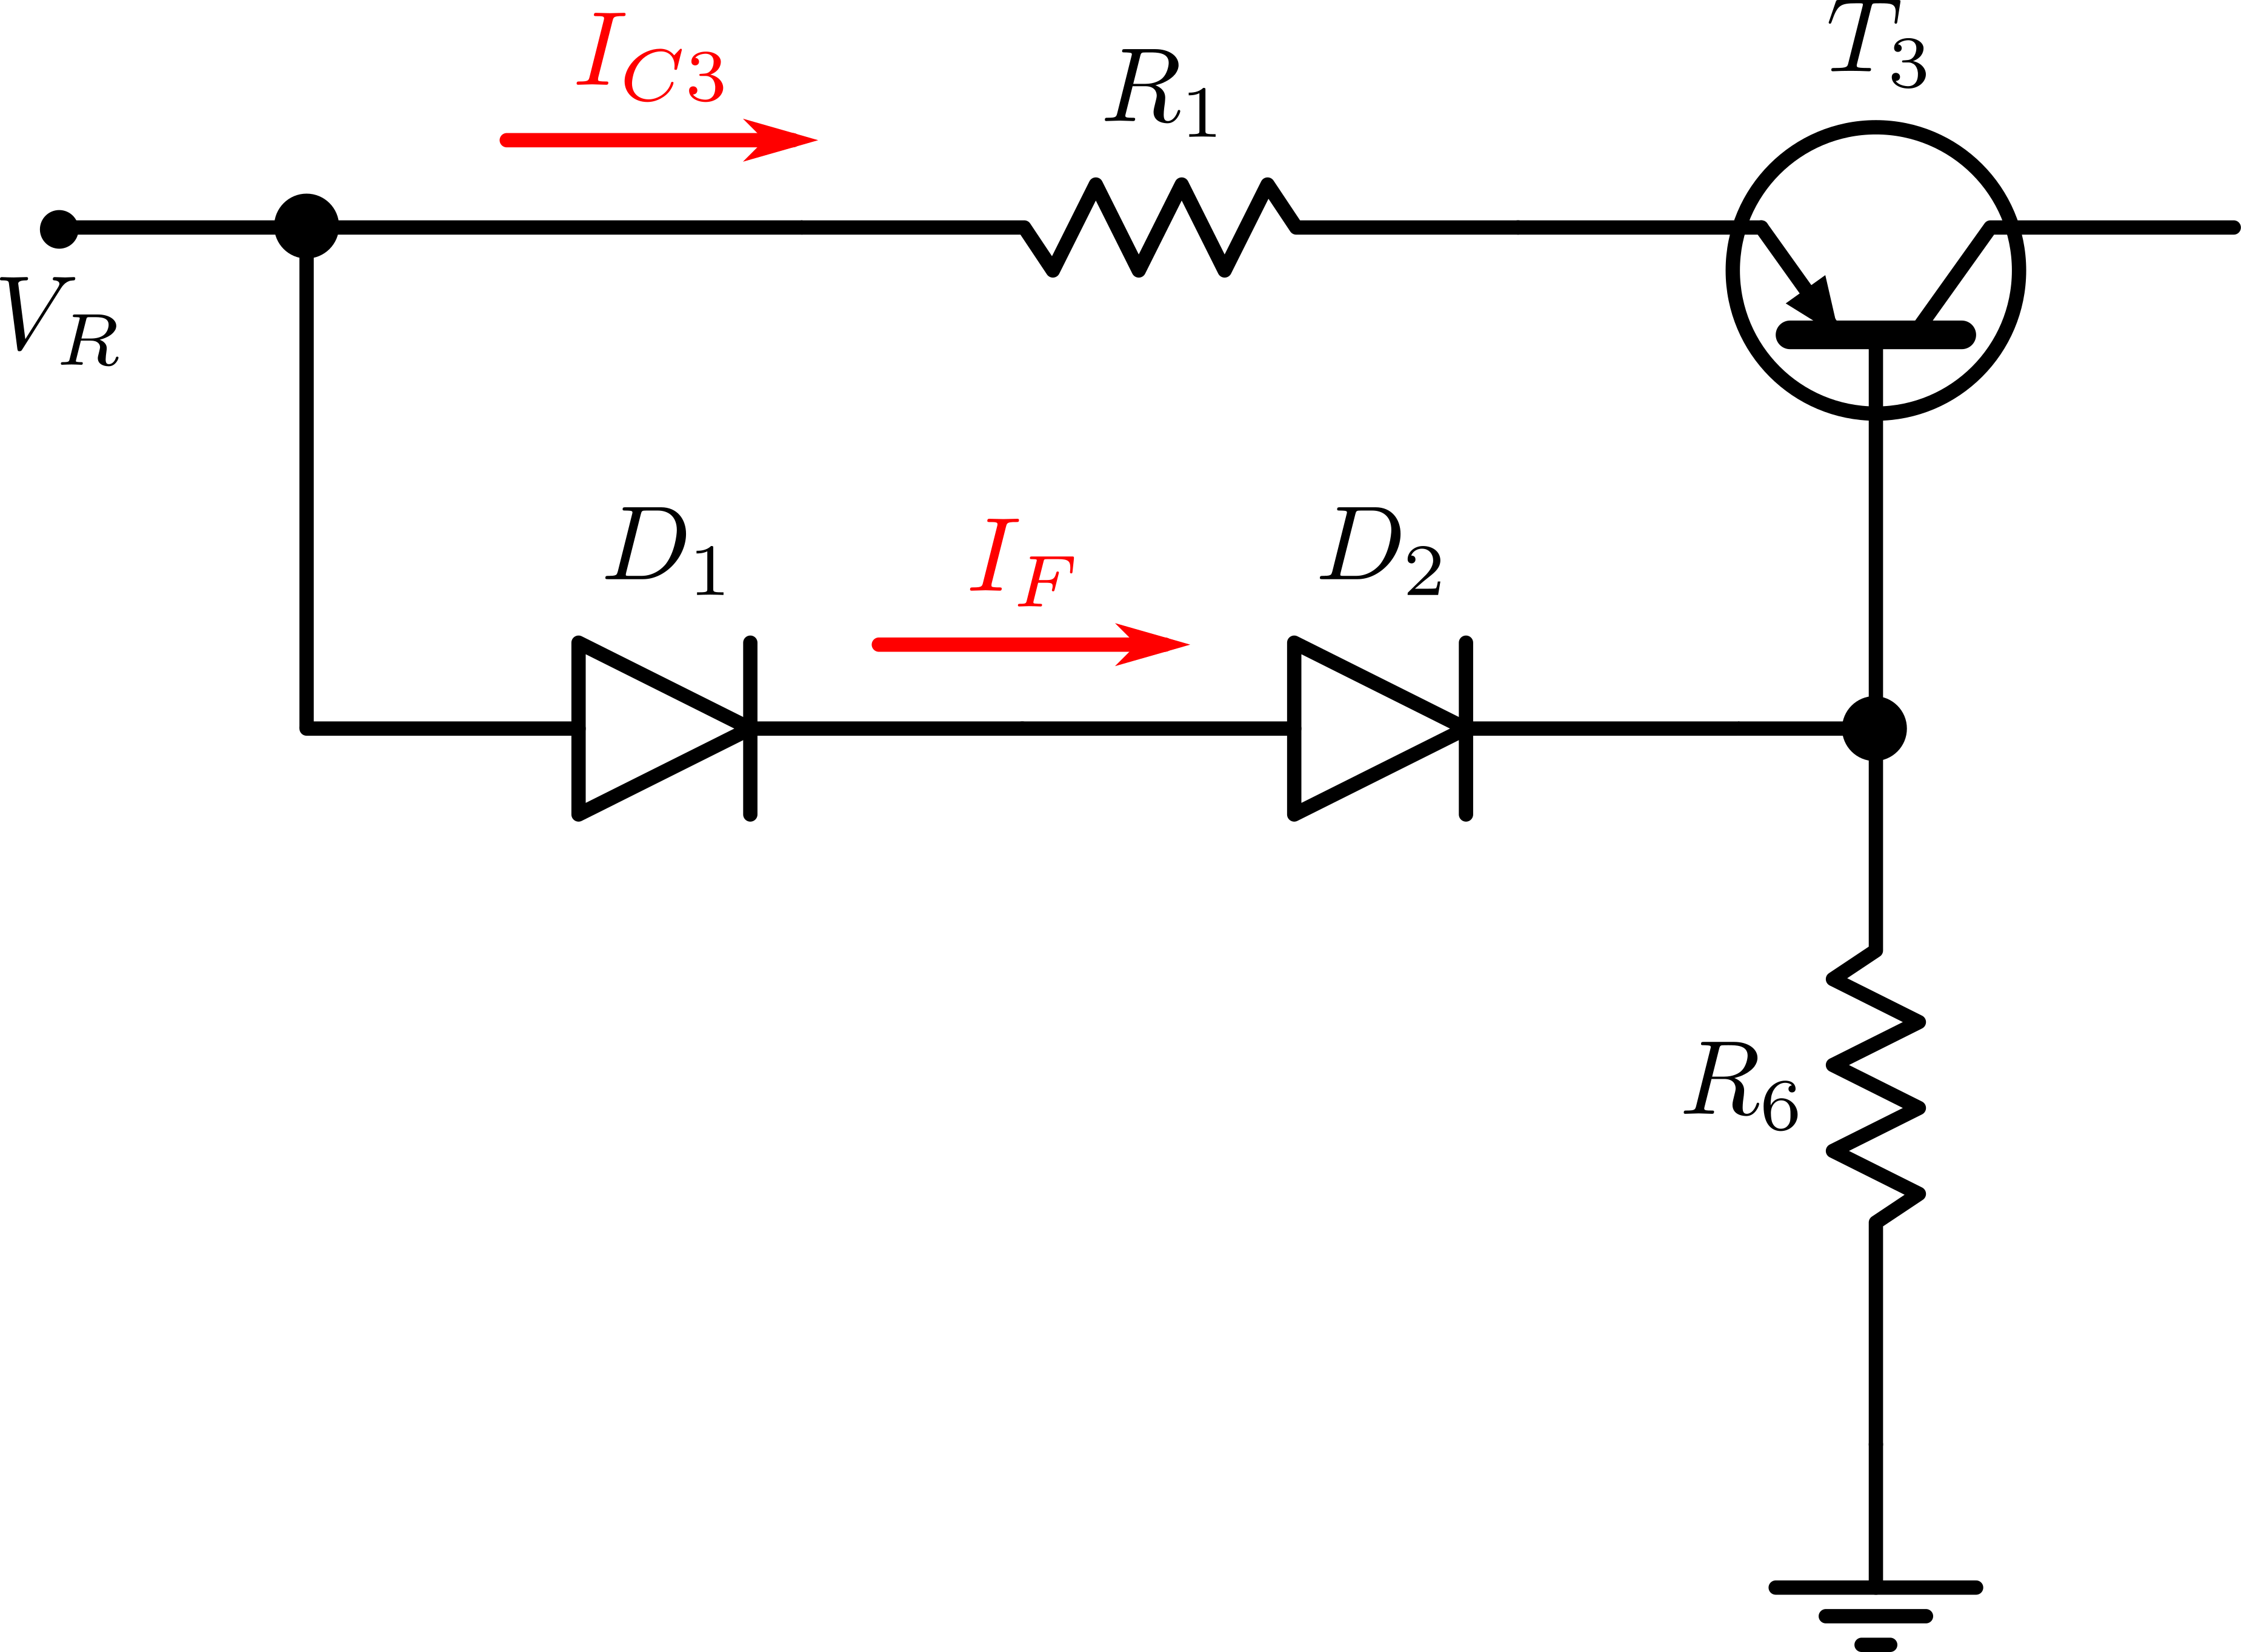
\includegraphics[scale=0.5]{Imagenes/PreRegulador.png}
\par\end{centering}
\caption{Circuito de pre-regulador}

\end{figure}

Se considera un margen para la corriente m\'axima, tomando $I_O = 1.6A$. Siendo $\beta2_{MIN} = 500$ (en DC), se calcula la corriente que se le debe proveer a la base de $T_2$ en el peor caso:

\[
I_{B2} = \frac{I_{C2}}{\beta2_{MIN}} = \frac{I_O}{\beta2_{MIN}}= 3.2mA
\]

Entonces $I_{C3}$ ser\'a la $I_{B2}$ m\'axima. Dado que no hay requerimientos particulares para $T_3$, por simplicidad en la selecci\'on de componentes se utiliz\'o  $T_3 = BC327$, cuyo $\beta3_{MIN} = 100$ por lo que podremos luego despreciar la corriente de base para los c\'alculos. Planteando la malla comprendida por $R_1$, $BE_3$ y los diodos $D_1$ y $D_2$, se despeja el valor de $R_1$:

\[
2V_D - V_{{BE3}_{ON}} - I_{C3}R_1 = 0
\]

\par
En la ecuaci\'on anterior se observa que la corriente $I_{C3}$ resulta independiente de las variaciones de la entrada $V_R$. Se toma $V_D = V_{{BE}_{ON}} = 0.7V$. Como s\'olo se requiere que $D_1$ y $D_2$ est\'en correctamente polarizados para dar las ca\'idas de tensi\'on $V_D$ consideradas, y no disipar\'an una potencia apreciable, se elijen $D_1 = D_2 = 1N4148$ por simplicidad. Entonces:

\[
\frac{2V_D - V_{{BE3}_{ON}}}{I_{C3}} = R_1 = 218.75\Omega
\]

Como se tom\'o una $I_O$ m\'axima mayor a la nominal para tener un margen, se normaliza sin problemas $R_1$ hacia arriba, entonces:
\[
R_1(N) = 220\Omega
\]
Tomando una corriente de polarizaci\'on en directa para los diodos de $I_F = 5mA$, se tiene (despreciando la corriente de base de $T_3$):

\begin{equation}
V_R - 2V_D - I_FR_6 = 0
\label{eqn:R6_relation}
\end{equation}

Para definir la m\'inima $V_R$, se comsidera el caso donde el circuito entrega la m\'axima corriente para la m\'axima $V_O$, de manera tal que los transistores sigan funcionando en modo activo. Para ello se plantea:

\[
V_R > V_{O_{MAX}} + I_{O_{MAX}}R_A + V_{BE2_{ON}} + V_{CE3_{SAT}} + V_D
\]
Siendo de las hojas de datos de los transistores $V_{BE2_{ON}} = 1.8V$ y $V_{CE3_{SAT}} = 0.7V$, con $V_D = 0.7V$. Como se ver\'a en el dise\~no de la protecci\'on, $R_A$ tendr\'a un valor del orden de $1\Omega$, por lo que entonces se tiene:
\[
V_R > 10V + 1.5V + 1.8V + 0.7 + 0.7V = 14.7V
\]
Definiendo entonces una $V_R = 15V$. De la ecuaci\'on (\ref{eqn:R6_relation}) podemos despejar ahora el valor de $R_6$:
\[
\frac{V_R - 2V_D}{I_F} = R_6 = 2.72K\Omega \Longrightarrow R_6(N) = 2.7K\Omega
\]

\subsection{Generador}

\begin{figure}[!ht]
\begin{centering}
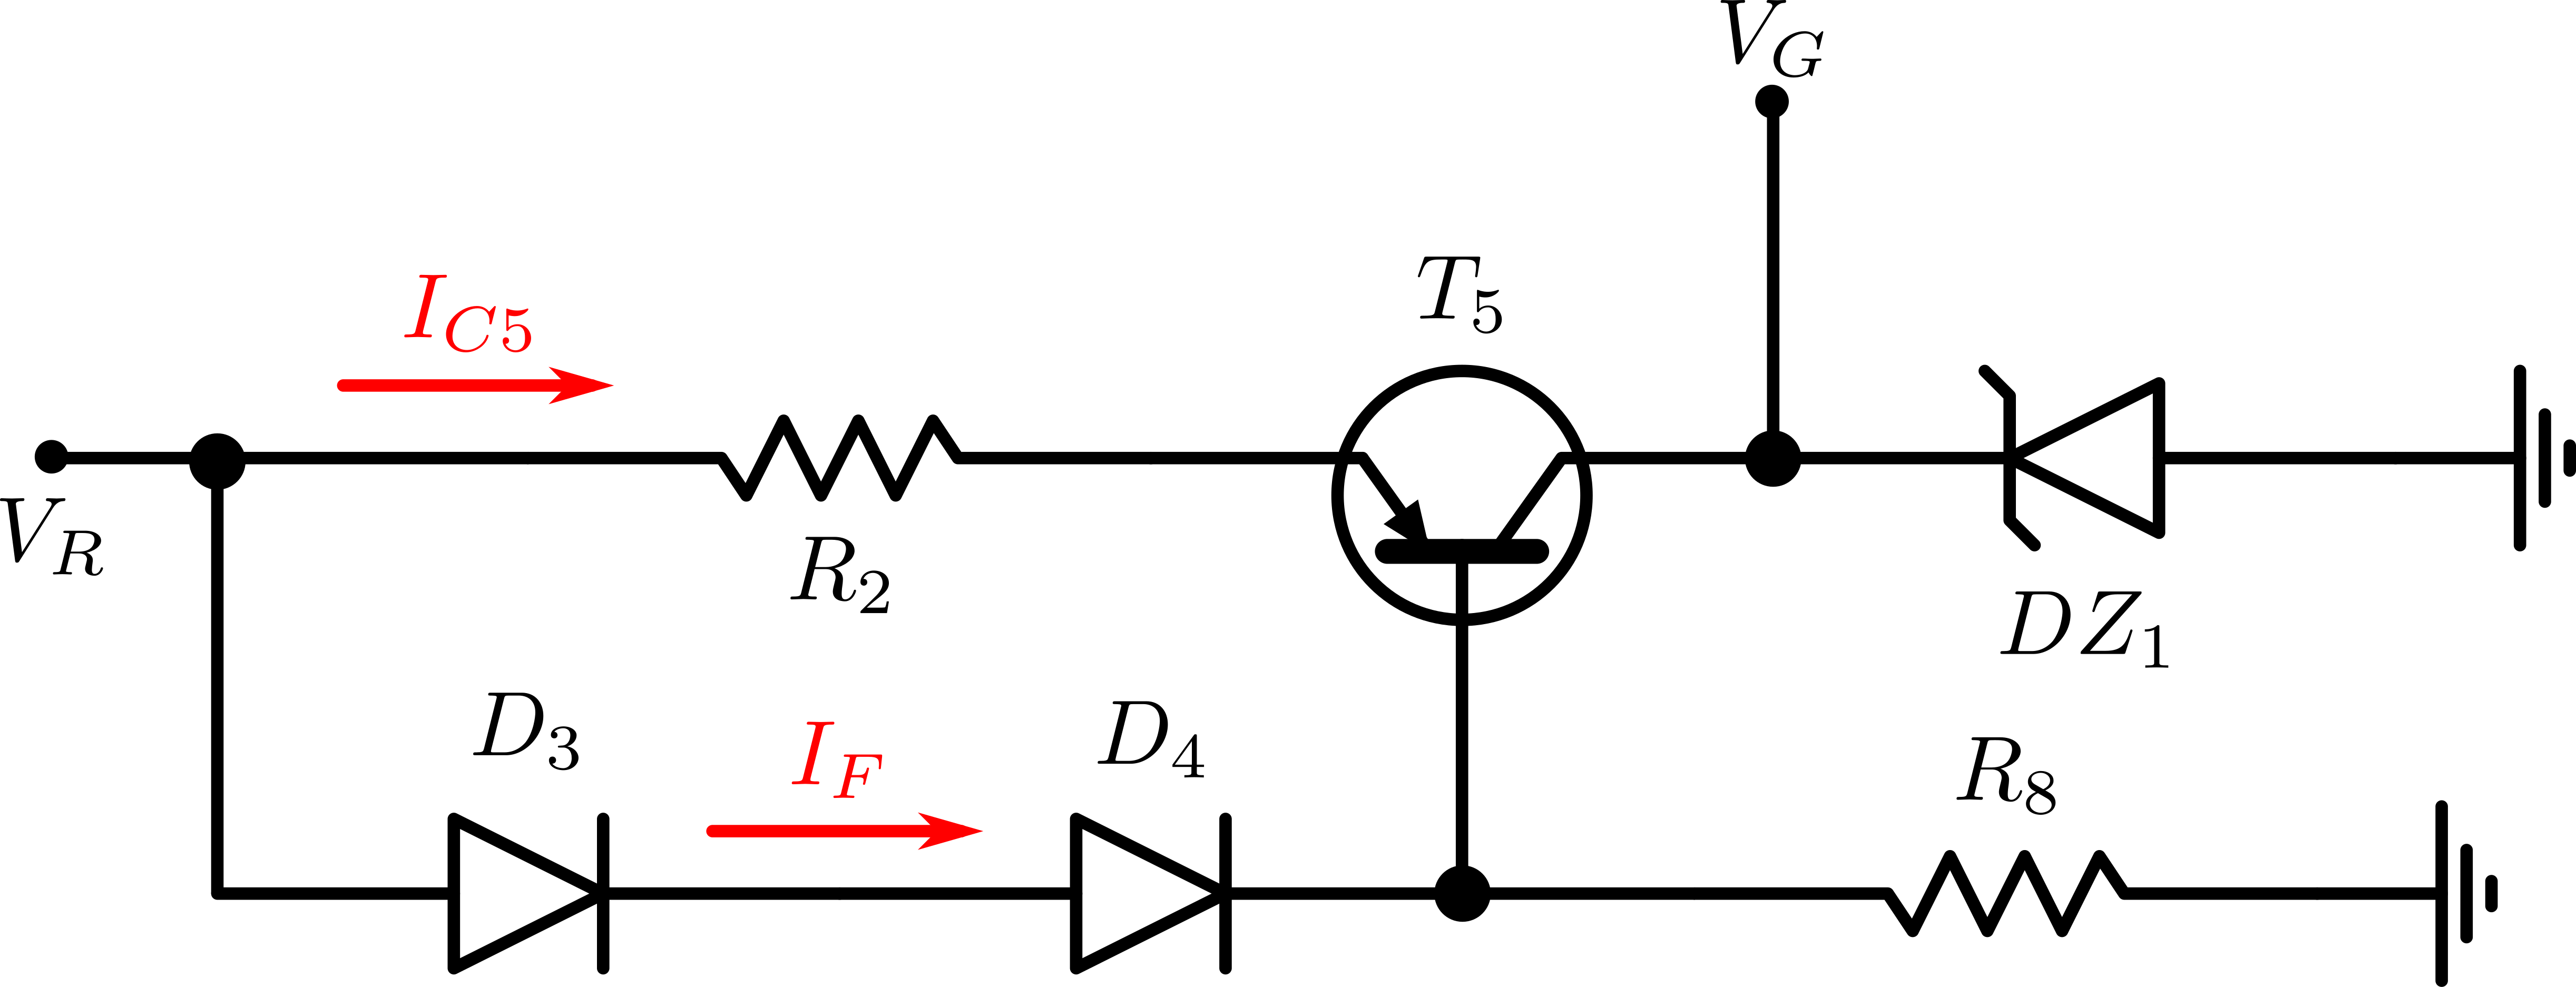
\includegraphics[scale=0.34]{Imagenes/Generador.png}
\par\end{centering}
\caption{Circuito del generador}

\end{figure}

Realizando un planeto similar al pre-regulador, se seleccionan $D_3 = D_4 = 1N4148$. Se fija una corriente $I_{C5}$, de manera que el diodo zener reciba una corriente constante, y por ende la $V_Z$ no sufra variaciones importantes. Para no requerir una entrada $V_R$ m\'as grande, se utiliz\'o un diodo zener de baja tensi\'on de regulaci\'on, en este caso $V_Z = 2.7V$, donde el $DZ_1 = 1N5223$. Con la ecuaci\'on de malla:
\[
2V_D - V_{BE5_{ON}} - I_{C5}R_2 = 0
\]
Para el zener, de la hoja de datos del fabricante, se tiene que $I_{ZK} = 0.25mA$. Se supone una corriente de polarizaci\'on inversa de $I_R = 5mA$ (de manera tal que sea mayor a la m\'inima $I_{ZK}$ mencionada), que ser\'a aproximadamente igual a $I_{C5}$. Se despeja entonces $R_2$ de la ecuaci\'on anterior y con la corriente impuesta se calcula su valor:
\[
\frac{2V_D - V_{BE5_{ON}}}{I_{C5}} = R_2 = 140\Omega \Longrightarrow R_2(N) = 120\Omega
\]
Dado que el circuito es similar al del pre-regulador, se utiliz\'o por simplicidad el mismo transistor PNP, es decir que $T_5 = BC327$.

Con el mismo criterio, se supone una $I_F = 5mA$, de manera tal que obtenemos para $R_8$ el mismo valor que $R_6$, entonces $R_8(N) = 2.7K\Omega$.

\newpage

\subsection{Detector}

Analizando el circuito por realimentaci\'on negativa, se pueden identificar los bloques de 'amplificador', 'realimentador' y 'generador':

\begin{figure}[!ht]
\begin{centering}
\includegraphics[scale=0.34]{Imagenes/CircuitoConFeed.png}
\par\end{centering}
\caption{An\'alisis por realimentaci\'on negativa}

\end{figure}

A la salida se muestrea tensi\'on y a la entrada se suma tensi\'on, por lo que el par\'ametro estabilizado resulta:
\[
PE = \frac{V_O}{V_G} = \frac{1}{f} \cdot \frac{|T|}{1+|T|}
\]
Donde $|T| = |a\cdot f|$. Asumiendo que $|T|$ es lo suficientemente grande:
\[
\frac{V_O}{V_G} \simeq \frac{1}{f}
\]

Por lo que hallando $f$ tendremos la relaci\'on entre la tens\'on de salida en funci\'on de la del generador, que es la $V_Z$.
\[
f = \left. \frac{\textrm{Magnitud que sumo}}{\textrm{Magnitud que muestreo}} \right|_{\textrm{Par\'ametro com\'un a la entrada = 0}}
\]
\\
Para hallar $f$ planteamos el cuadripolo correspondiente:

\begin{figure}[!ht]
\begin{centering}
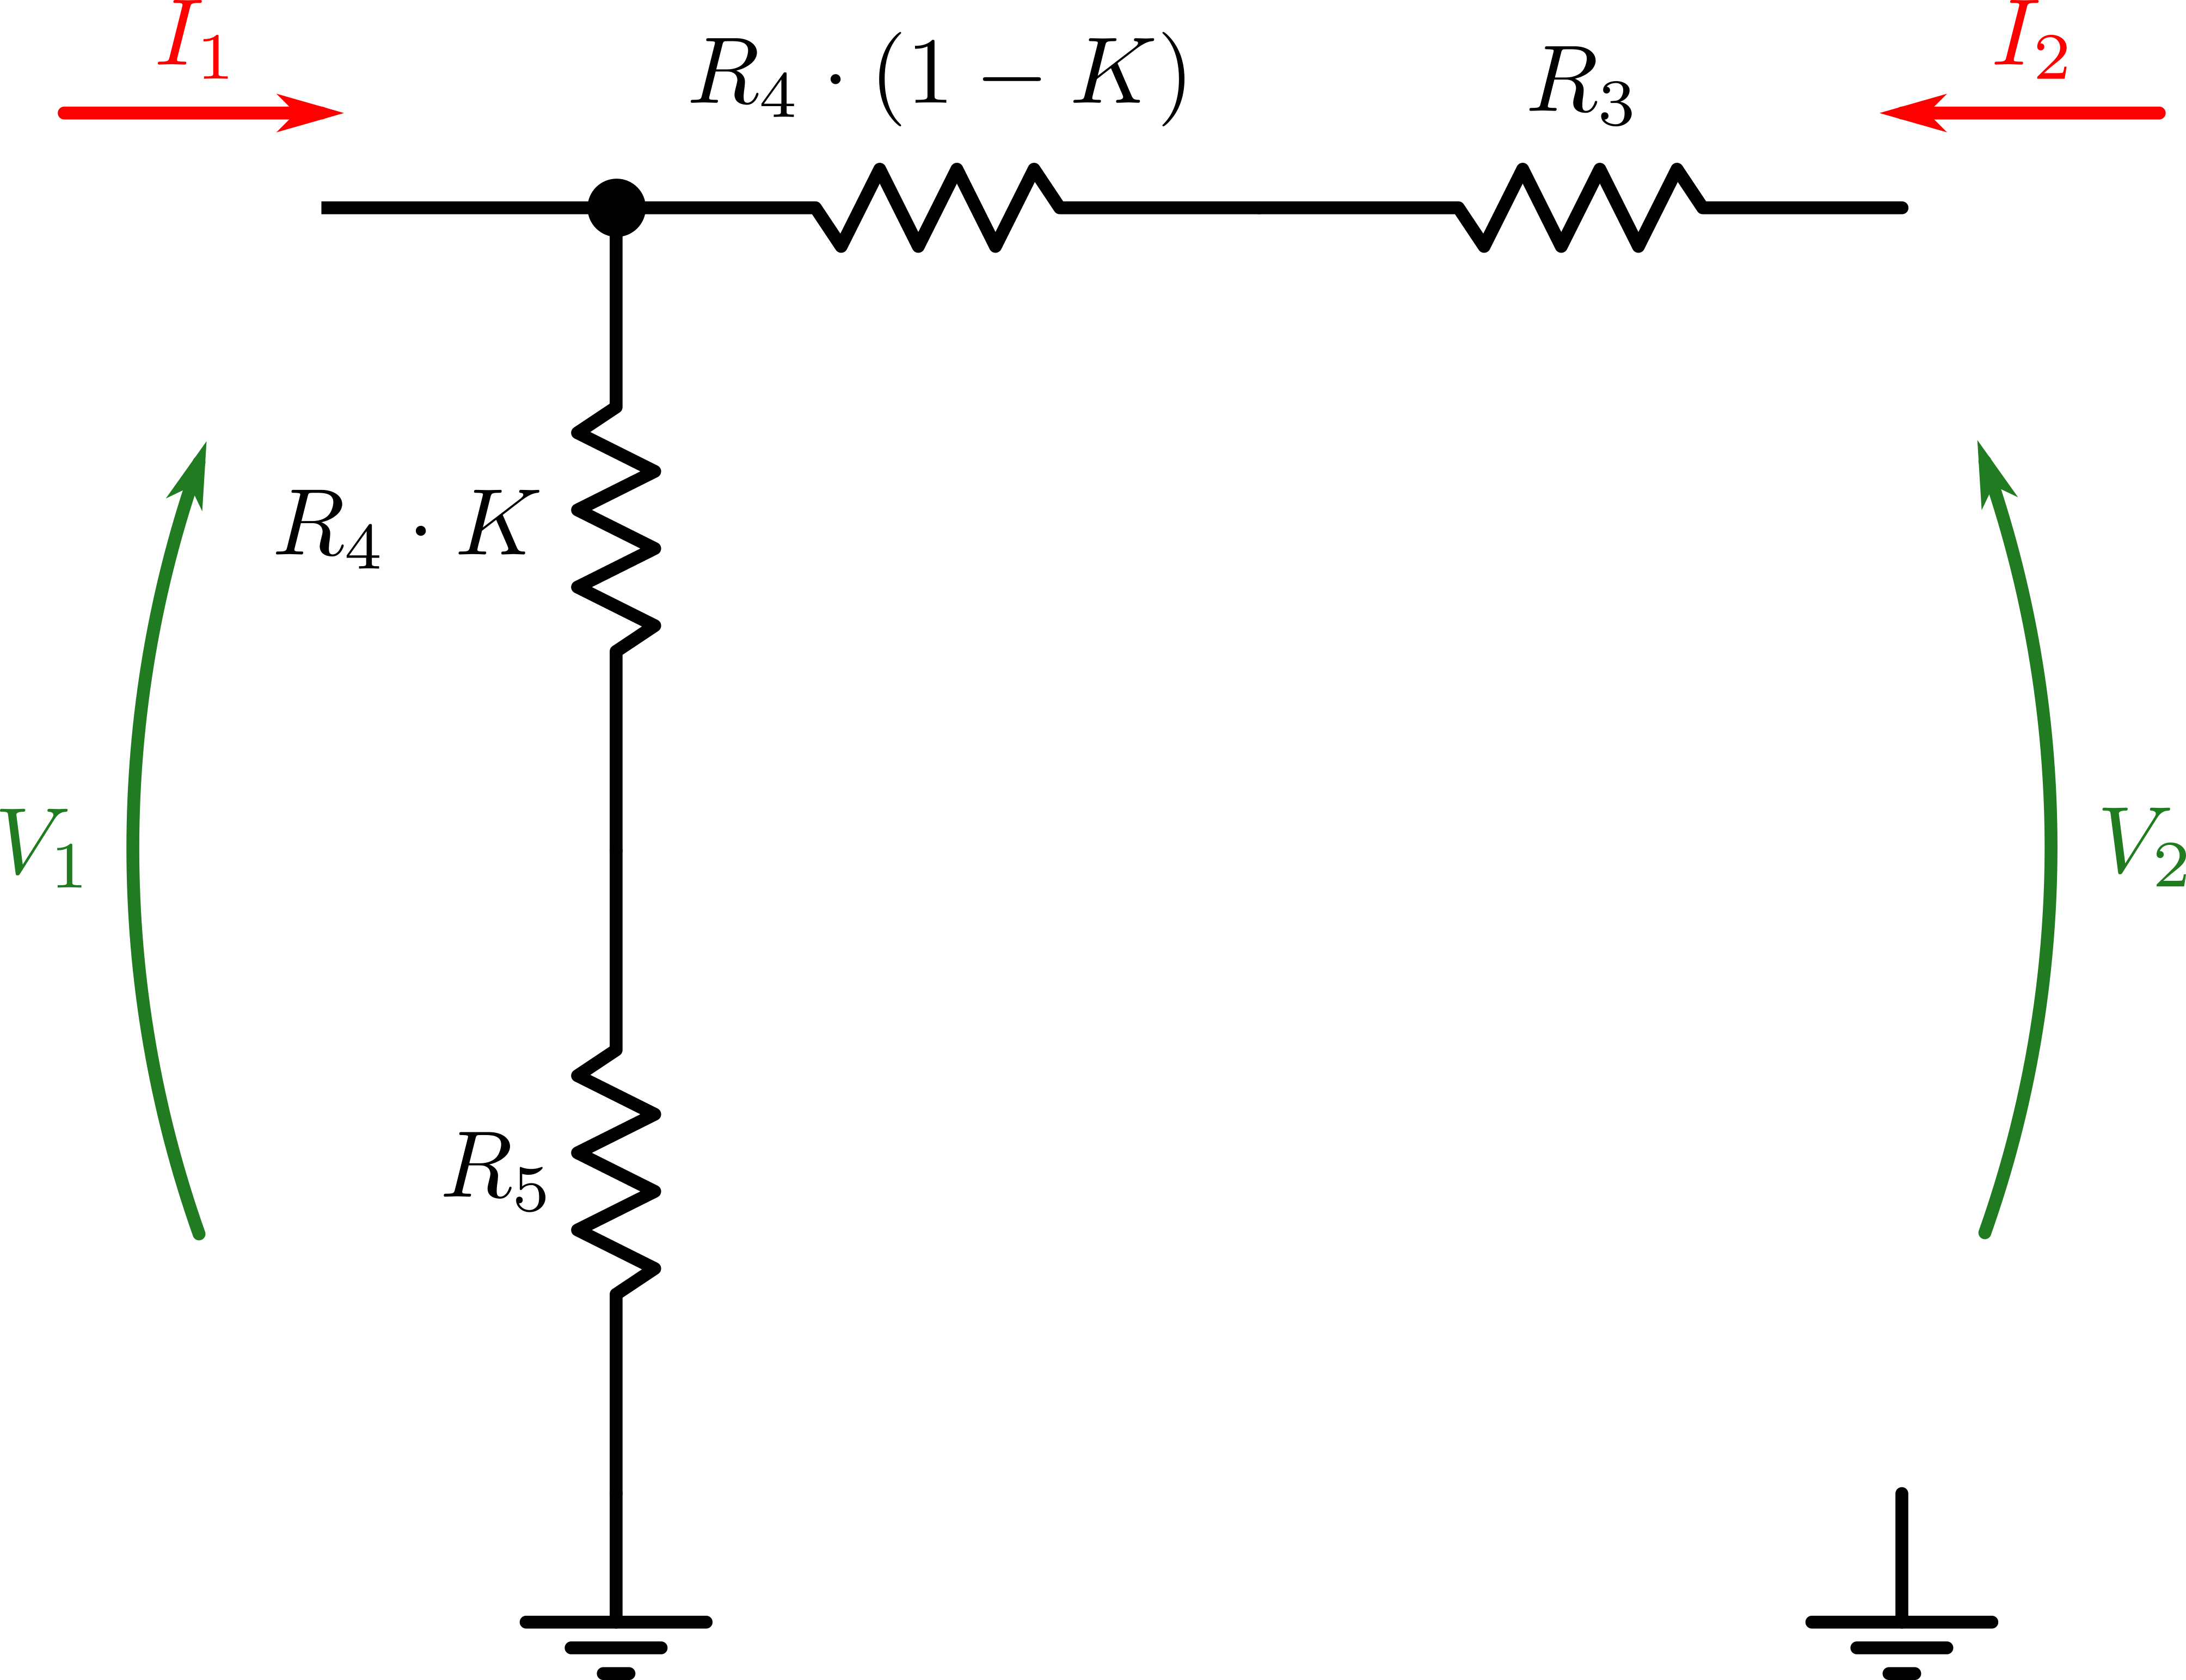
\includegraphics[scale=0.34]{Imagenes/CuadripoloF.png}
\par\end{centering}
\caption{Modelo del cuadripolo $f$}

\end{figure}

Dado que $R_4$ es un potenci\'ometro, se la representa en dos partes ($0 \leq K \leq 1$). Entonces se tiene:
\[
f = \left. \frac{V_1}{V_2} \right|_{I_1=0} = \frac{R_4 \cdot K + R_5}{R_3 + R_4 + R_5}
\]
Seg\'un $K$ valga 0 o 1, tendremos $V_O$ m\'axima o m\'inima:

\[
\left\lbrace
\begin{array}{l}
V_{O_{MIN}} = V_G \cdot \dfrac{R_3+R_4+R_5}{R_4+R_5}\\ \\
V_{O_{MAX}} = V_G \cdot \dfrac{R_3+R_4+R_5}{R_5}
\end{array}
\right.
\]

Para el dise\~no, mediante correcciones con simulaci\'on y prueba en protoboard, se tom\'o un margen m\'as amplio para $V_O$ respecto del nominal. Se utiliz\'o entonces como resultado de dichas pruebas un rango $3.9V \leq V_O \leq 10.4V$. Dividiendo ambas ecuaciones se puede despejar $R_5$ en funci\'on de $R_4$, resultando:
\[
R_5 = \frac{3}{5} \cdot R_4
\]
Tomando un potenci\'ometro nominal, se define $R_4(N) = 10K\Omega$, por lo que resulta $R_5 = 6K\Omega$. Normalizando, se tiene:
\[
R_5(N) = 12K\Omega \textrm{ // } 12K\Omega
\]
De la segunda ecuaci\'on se despeja $R_3$, obteniendo:
\[
\left(\frac{V_{O_{MAX}}}{V_G}\right)R_5 - R_5 - R_4 = R_3 \Longrightarrow R_3 = 7.11K\Omega
\]
Normalizando se tiene que: 
\[
R_3(N) = 6.8K\Omega + 330\Omega
\]

\subsection{Amplificador de error}

\begin{figure}[!ht]
\begin{centering}
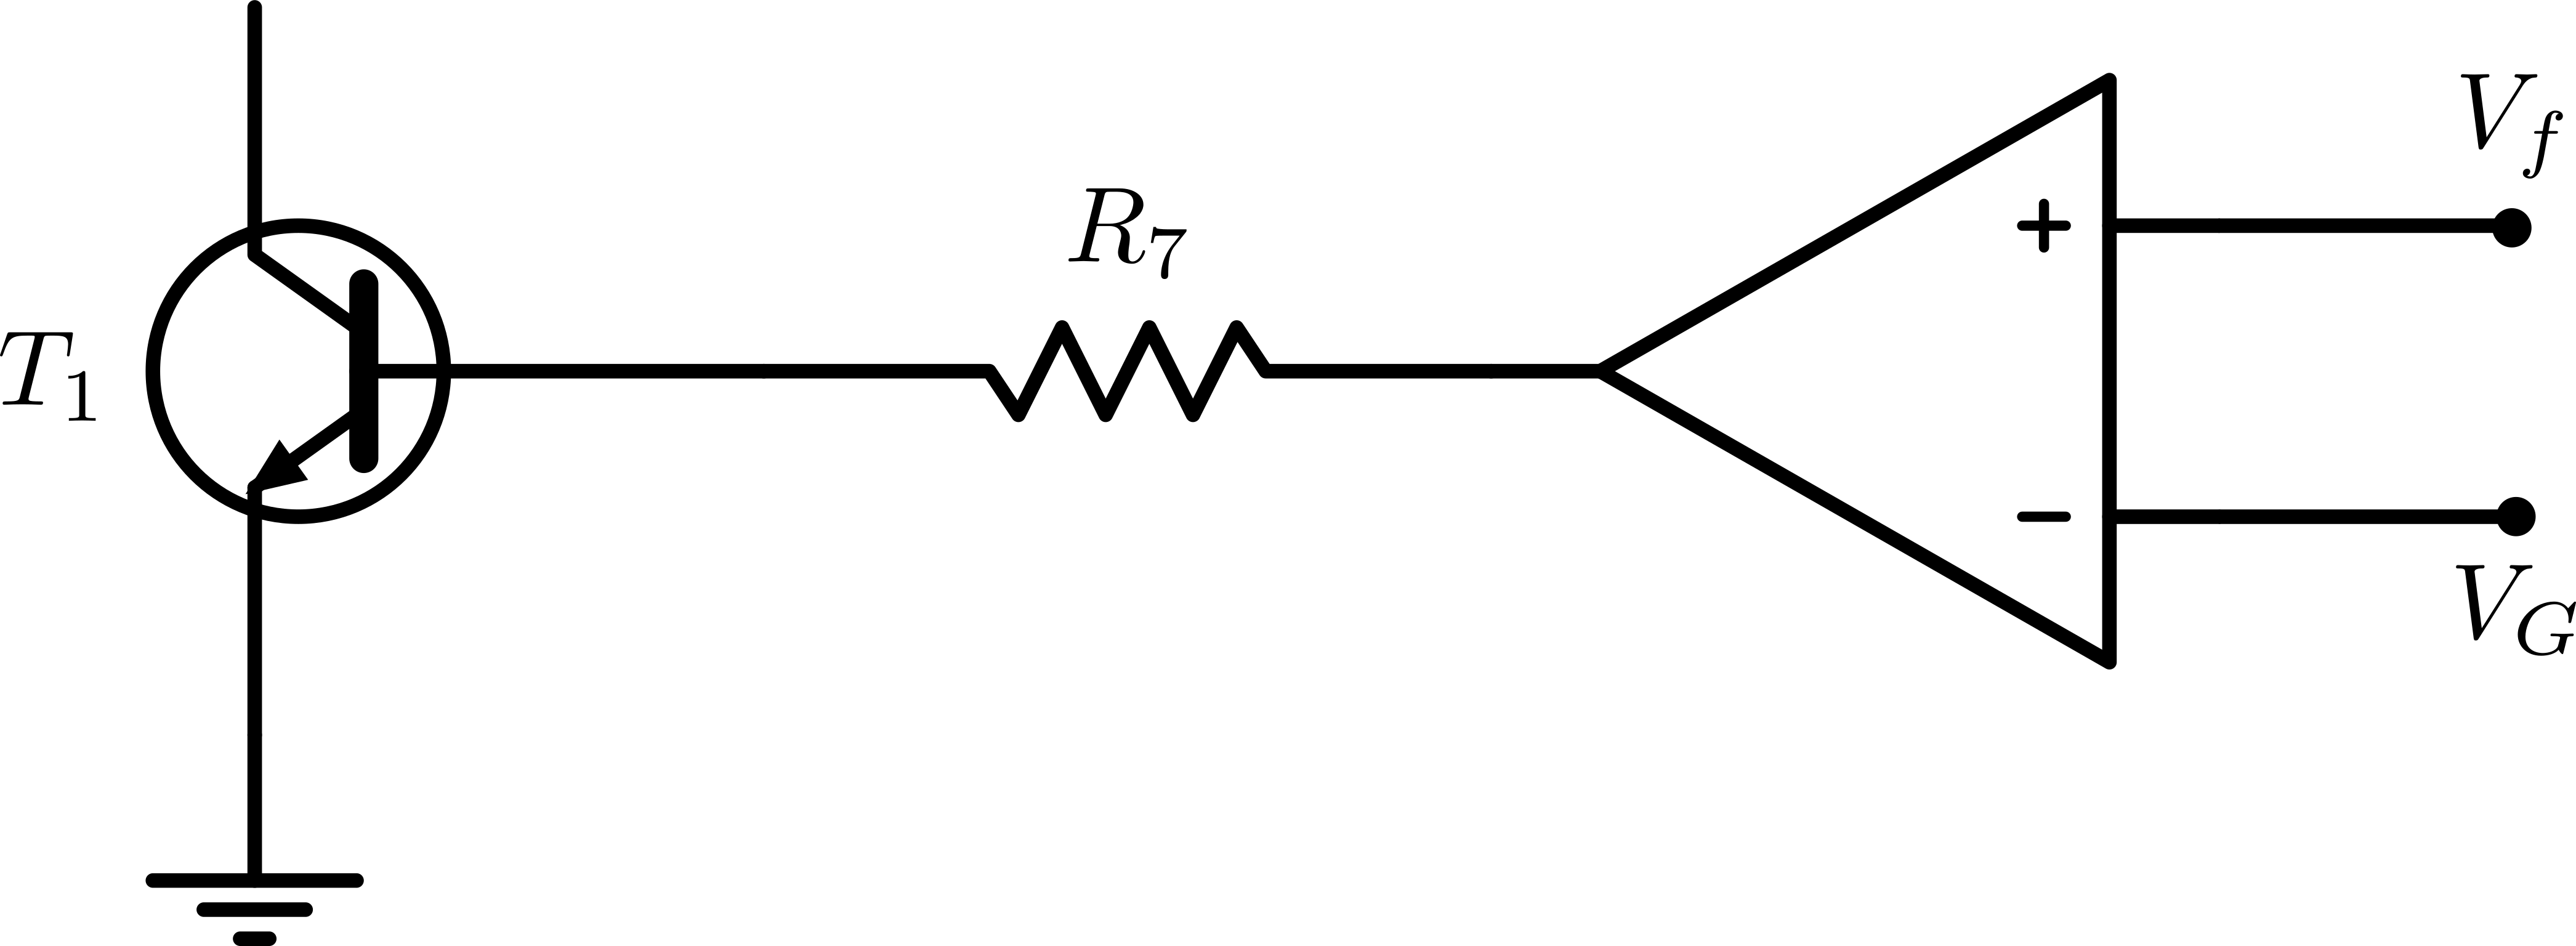
\includegraphics[scale=0.5]{Imagenes/CircuitoError.png}
\par\end{centering}
\caption{Circuito del amplificador de error}

\end{figure}


El amplificador de error se compone del operacional m\'as el transistor $T_1$. Dado que a la entrada de la fuente s\'olo se dispone de una s\'ola tensi\'on $V_R$ positiva, se debi\'o utilizar un operacional que pueda funcionar con fuente simple. Adem\'as, su ganancia a lazo abierto debe ser grande para que la ganancia de lazo $|T|$ sea grande, y valga la suposici\'on realizada anteriormente para el diseño del detector. Tambi\'en el ancho de banda del operacional no debe ser muy grande, para reducir la posibilidad de tener oscilaciones a la salida del circuito (esto \'ultimo se trata en la secci\'on de ganacia de lazo y su compensaci\'on).\par
En base a esto, el operacional seleccionado es el $LM358$.\par
El transistor $T_1$ cumple la funci\'on de realizar la inversi\'on para que la realimentaci\'on resulte negativa (conectando al operacional como no inversor). Por otra parte, al estar configurado como emisor com\'un, aumenta m\'as la ganancia de lazo. \par
El transistor seleccionado finalmente fue $T_1 = BC548C$. Dado su alto valor de $\beta$ no exige corriente a la salida del operacional.\par
La resistencia $R_7$ se añadi\'o para que el operacional entregue una tensi\'on mayor a la $V_{BE1_{ON}}$, de manera tal que se encuentre con un cierto margen por encima de los $0V$, dado que se lo aliment\'o con fuente simple. Se determin\'o un valor adecuado para ella mediante la simulaci\'on, de manera tal que el circuito funcionara correctamente, resultando: 
\[
R_7(N) = 100K\Omega
\]
\newpage

\subsection{Protecci\'on}

\begin{figure}[!ht]
\begin{centering}
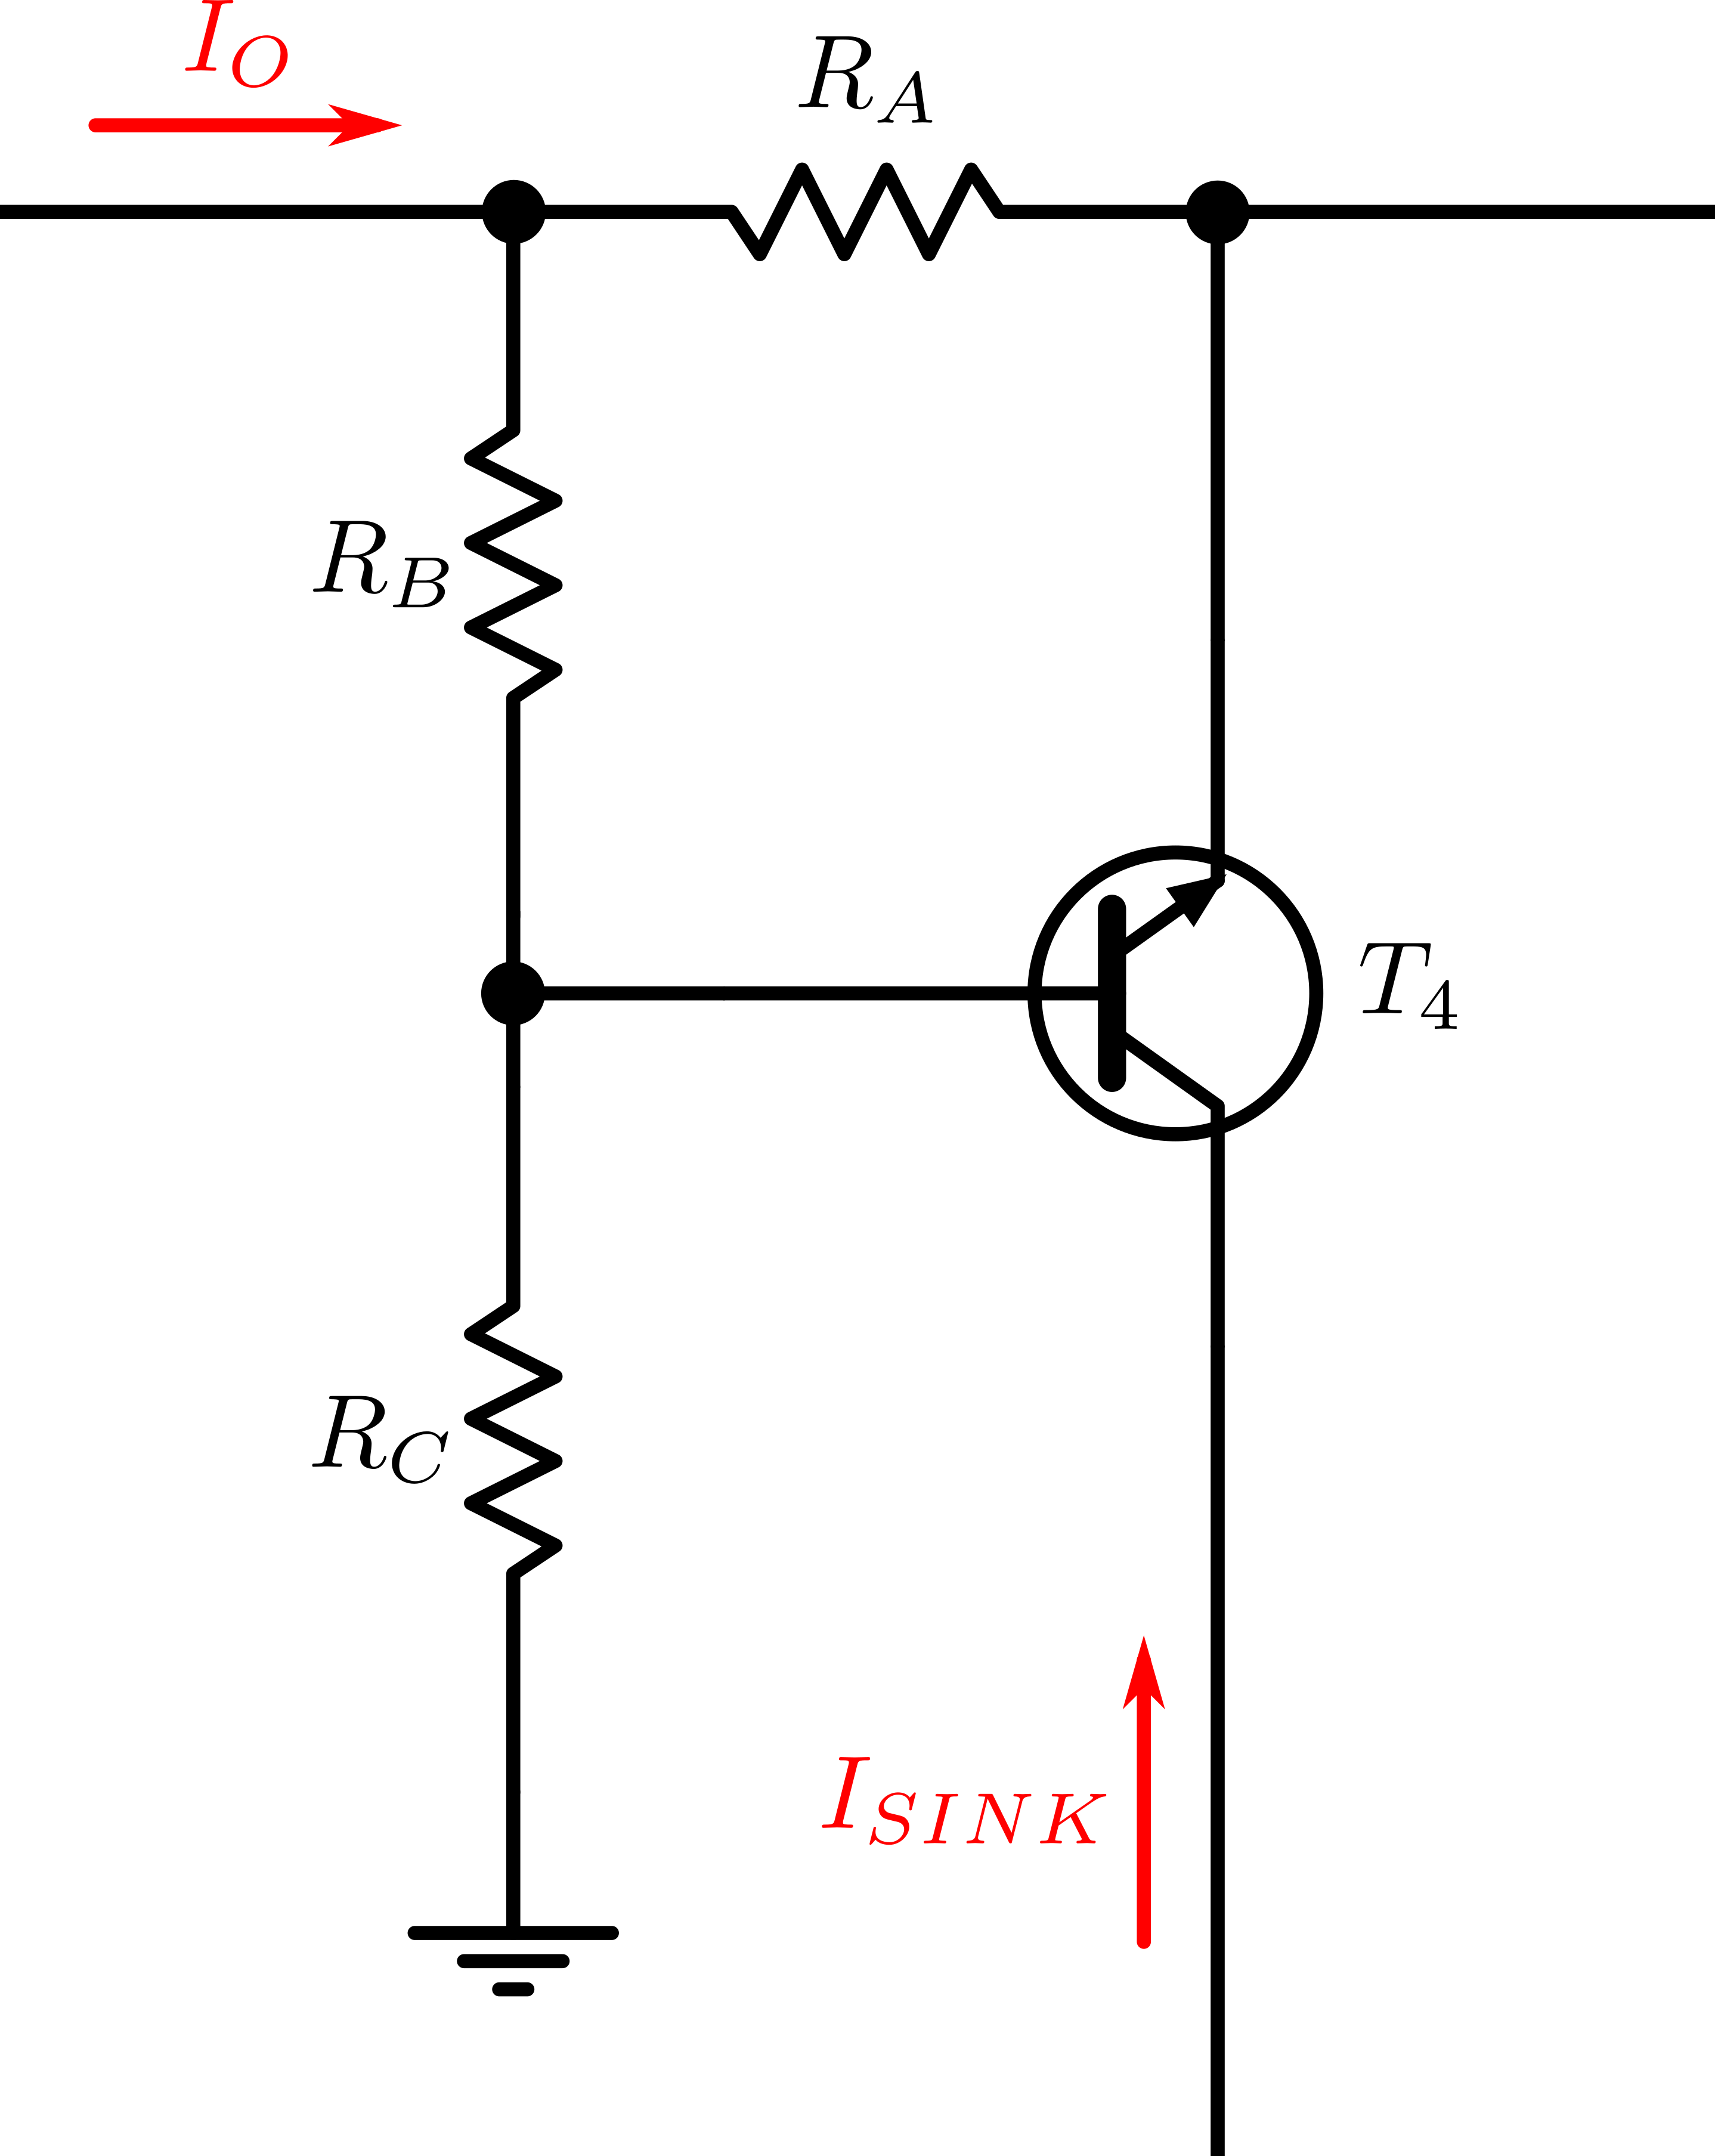
\includegraphics[scale=0.4]{Imagenes/Proteccion.png}
\par\end{centering}
\caption{Circuito de la protecci\'on Foldback}

\end{figure}

La protecci\'on utilizada se denomina Foldback. Mientras la $R_L$ sea mayor a la m\'inima en regulaci\'on, la tensi\'on $V_{BE4} < V_{BE4_{ON}}$, por lo que $T_4$ no se enciende y la protecci\'on no incide en el circuito. Cuando se disminuye la carga $R_L$ por debajo de la m\'inima que puede conectarse en regulaci\'on, el lazo de realimentaci\'on se abre y el transistor $T_4$ comienza a conducir, tomando parte de la corriente que va a la base de $T_2$ (dado que $I_{PRE-REG}$ es constante) que es la indicada como $I_{SINK}$, y la tensi\'on y corrientes de salida pasan a estar determinados por una expresi\'on lineal, donde a medida que la $V_O$ disminuye, la $I_O$ tambi\'en lo hace. De esta manera, veremos que la $I_{O_{CC}} < I_{O_{MAX}}$.\par
Para observar esto, se plantea la malla que contiene a $V_{BE4_{ON}}$:
\[
(V_O + I_O \cdot R_A)\cdot \frac{R_B}{R_B+R_C} + V_{BE4_{ON}} = I_OR_A
\]
Como no se requiere amplificar corriente sino que el objetivo es sensar $I_O$ y derivar corriente de la base de $T_2$, se elije $T_4 = BC337$, cuyo $\beta_{MIN} = 100$ (se tiene entonces que $V_{BE4_{ON}} = 0.7V$). Para simplificar la notaci\'on, llamamos $\alpha = \dfrac{R_B}{R_B+RC}$. Despejando $I_O$ resulta:

\begin{equation}
I_O = \frac{V_O \cdot \alpha + V_{BE4_{ON}}}{R_A(1-\alpha)}
\label{eqn:io_fb}
\end{equation}

EL gr\'afico caracter\'istico resultante es el siguiente:

\begin{figure}[!ht]
\begin{centering}
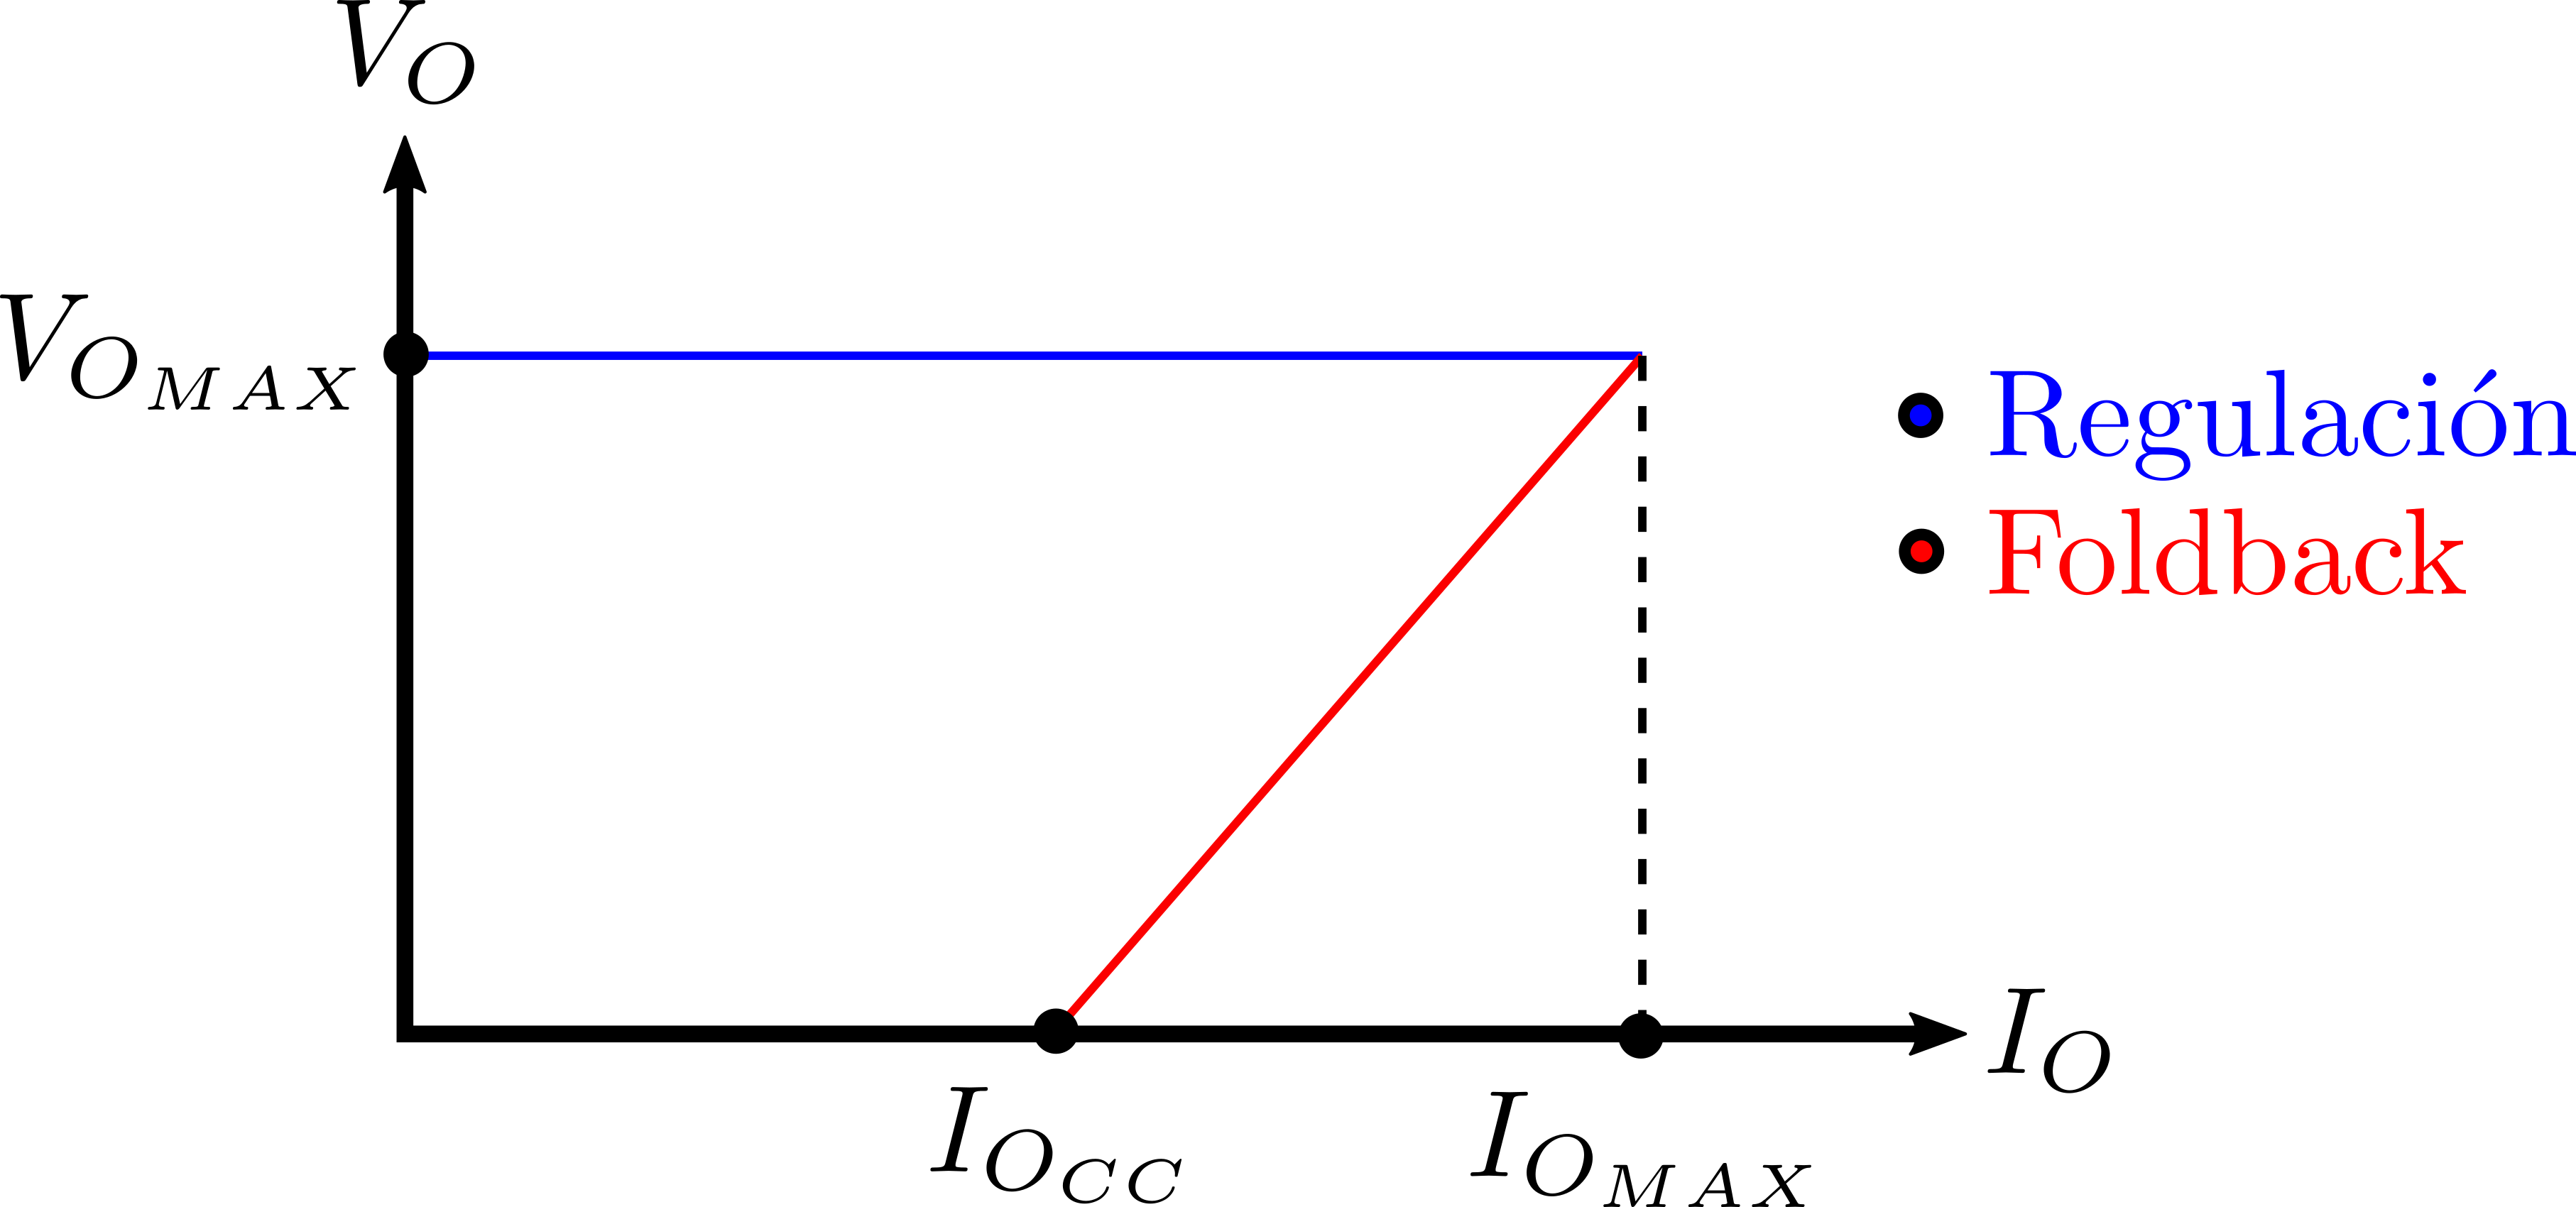
\includegraphics[scale=0.6]{Imagenes/FB_Generico.png}
\par\end{centering}
\caption{Caracter\'istica de salida ideal con protecci\'on Foldback}

\end{figure}

Como la funci\'on de $R_A$ es \'unicamente sensar la corriente de salida $I_O$, no debe ser muy grande para no perder demasiada potencia en ella. Teniendo en cuenta que:

\begin{equation}
\left. R_{L_{MIN}} \right|_{REG} = \left. \frac{V_{O_{MAX}}}{I_{O_{MAX}}} \right|_{REG} = 6.4\Omega
\label{eqn:RL_MIN}
\end{equation}

Un criterio adecuado para seleccionar $R_A$ es que sea 10 veces menor a la $R_L$ m\'inima en regulaci\'on. Pero como puede observarse de la ecuaci\'on (\ref{eqn:RL_MIN}), al estar definidos $V_{O_{MAX}}$ e $I_{O_{MAX}}$ en regulaci\'on, queda formada una relaci\'on de compromiso entre $\alpha$ y $R_A$, que tambi\'en en consecuencia definir\'a la $I_{O_{CC}}$, y por ende el punto donde la potencia disipada en $T_2$ sea m\'axima (esto \'ultimo se tratar\'a en la secci\'on siguiente). Si de la ecuaci\'on (\ref{eqn:RL_MIN}) despejamos $\alpha$:

\begin{equation}
\alpha = \frac{I_O \cdot R_A - 0.7V}{V_O + I_O \cdot R_A}
\label{eqn:alpha}
\end{equation}

De la ecuaci\'on (\ref{eqn:alpha}) vemos que, en referencia a lo mencionado anteriormente, si se reemplaza por $V_{O_{MAX}}$ e $I_{O_{MAX}}$, $R_A$ no puede valer cualquier cosa sino que tendr\'a un valor m\'inimo, tal que $\alpha > 0$ (porque es un cociente de un divisor resistivo).\par
Seleccionando $R_A = 1\Omega$, con la $I_{O_{MAX}} = 1.6A$ que se dio de margen previamente, se tiene que la potencia m\'axima que debe disipar $R_A$ es $R_A \cdot I^2_{O_{MAX}} = 2.56W$. Por lo que normalizando se tiene:
\[
R_A(N) = 1\Omega - 3W
\]
Reemplazando $V_{O_{MAX}}$, $I_{O_{MAX}}$ y $R_A(N)$ en la ecuaci\'on (\ref{eqn:alpha}) se obtiene:
\[
\frac{R_A \cdot I_{O_{MAX}}- 0.7V}{V_{O_{MAX}} + R_A \cdot I_{O_{MAX}}} = \alpha = 0.076
\]
Teniendo $\alpha$, se seleccionan en forma simple $R_B$ y $R_C$ para el divisor resistivo, de forma tal que:
\[
R_B(N) = 1K\Omega \hspace{2cm} R_C(N) = 12K\Omega
\]
Con el valor de $\alpha$ calculado, si $V_O = 0V$, la $I_O$ resultante es la de cortocircuito:
\[
I_{O_{CC}} = 0.76A
\]

\subsection{Disipaci\'on de potencia}

Teniendo ya el circuito con los componentes seleccionados, resta definir la potencia m\'axima que disipar\'a $T_2$ y si requiere o no un disipador. 
En general, la potencia que disipa el transistor $T_2$ est\'a dada por:

\begin{equation}
P_D(T_2) = V_{CE_2} \cdot I_O = (V_R - V_O - R_A \cdot I_O) \cdot I_O
\label{eqn:pdT2}
\end{equation}

A medida que se disminuye $R_L$ desde el infinito hasta la m\'inima de regulaci\'on, la $V_O$ se mantiene constante y la $I_O$ aumenta, por lo que la $PD_{T_2}$ va en aumento en forma mon\'otona. Cuando la $R_L < R_{L_{MIN}}$, se sale de la regulaci\'on y se entra en la recta de foldback. Mientras se sigue disminuyendo $R_L$, la $V_O$ comienza a disminuir por lo que la $V_{CE_2}$ aumenta; pero a su vez la $I_O$ disminuye. Si se reemplaza la expresi\'on de $I_O$ de la ecuaci\'on (\ref{eqn:io_fb}) de foldback, en la expresi\'on de potencia disipada (\ref{eqn:pdT2}):

\[
P_D(T_2) = \left( V_R - V_O - R_A \cdot \frac{V_O \cdot \alpha + 0.7V}{R_A(1-\alpha)}\right) \cdot \frac{V_O \cdot \alpha + 0.7V}{R_A(1-\alpha)}
\]  

Queda entonces la $P_D(T_2)$ como una funci\'on cuadr\'atica de $V_O$, con concavidad hacia abajo. Esto quiere decir que la potencia m\'axima se encuentra en la $V_O$ del v\'ertice de la par\'abola. En una ecuaci\'on cuadr\'atica general:

\[
ax^2 + bx + c \Longrightarrow x_v = -\frac{b}{2a} 
\]

Si se hace la distributiva de los t\'erminos de la expresi\'on de $P_D(T_2)$ y se los agrupa adecuadamente para tener el formato anterior con los coeficientes $a$, $b$, y $c$, se puede obtener la $V_{O_v}$ (donde estar\'a el m\'aximo de la $P_D(T_2)$):

\[
V_O \biggr|_{PD_{MAX}} = \frac{V_R \cdot \alpha \cdot (1-\alpha) - 0.7V \cdot (1+\alpha)}{2\alpha} = 1.97V
\]

Reemplazando en la expresi\'on de $I_O$ de la ecuaci\'on (\ref{eqn:io_fb}), se obtiene:

\[
I_O \biggr|_{PD_{MAX}} = 0.92A \Longrightarrow P_D(T_2) \biggr|_{MAX} = 11.14W
\]
 
Como la potencia m\'axima total que admite disipar el $TIP112$ es de $50W$, no hay inconveniente en utilizarlo. Con esta informaci\'on calculamos ahora la potencia m\'axima sin disipador que soporta el transistor. De la hoja de datos del fabricante se tiene que:

\[
T_j = 150^{\circ}C  \hspace{2cm} R_{\theta ja} = 62.5 \left( \frac{^{\circ}C}{W}\right) \hspace{2cm} R_{\theta jc} = 2.5 \left(\frac{^{\circ}C}{W}\right)
\] 
 
\[
\left\lbrace
\begin{array}{l}
R_{\theta ja}: \textrm{Resistencia t\'ermica entre juntura y ambiente} \\
R_{\theta jc}: \textrm{Resistencia t\'ermica entre juntura y carcasa del transistor}
\end{array}
\right.
\] 
 
\newpage 
 
Suponiendo una $T_a = 25^{\circ}C$, se tiene:

\[
P_D(T_2) \biggr|_{S/D} = \frac{T_j - T_a}{R_{\theta ja}} = 2W
\]
 
La potencia que se requiere disipar ($11.14W$) es entonces mayor a la m\'axima sin disipador, por lo tanto se necesita incorporarle uno. Con disipador, se tiene:

\[
P_D(T_2) \biggr|_{C/D} = \frac{T_j - T_a}{R_{\theta jc} + R_{\theta cd} + R_{\theta da}}
\]
 
\[
\left\lbrace
\begin{array}{l}
R_{\theta cd}: \textrm{Resistencia t\'ermica entre carcasa del transistor y disipador} \\
R_{\theta da}: \textrm{Resistencia t\'ermica entre disipador y el ambiente}
\end{array}
\right.
\] 

Utilizando pasta t\'ermica, la $R_{\theta cd} \approx 1(^{\circ}C/W)$, y la $R_{\theta da}$ m\'axima es la que se quiere averiguar para seleccionar el modelo de disipador a usar. Despej\'andola de la ecuaci\'on anterior:

\[
R_{\theta da} = \frac{T_j - T_a}{P_D(T_2)} - R_{\theta jc} - R_{\theta cd} = 7.45 \left(\frac{^{\circ}C}{W}\right)
\]
 
Se necesita entonces un disipador cuya $R_{\theta da}$ sea menor a la obtenida. Un disipador sencillo que cumple esta caracter\'istica con margen es el ZD9, cuya $R_{\theta da} = 3.8(^{\circ}C/W)$, por lo que se le incorpor\'o dicho disipador a $T_2$. 
 
\begin{figure}[!ht]
\begin{centering}
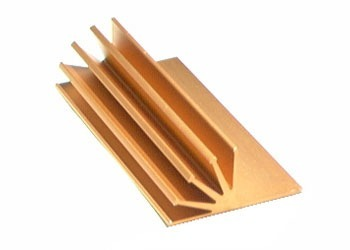
\includegraphics[scale=0.7]{Imagenes/ZD9.jpg}
\par\end{centering}
\caption{Disipador ZD9 comercial}

\end{figure}
 
\newpage 
 
\subsection{Ganancia de lazo - Compensaci\'on}

Utilizando LTSpice, se simula la respuesta en frecuencia de la ganancia de lazo, con el script provisto por la c\'atedra. El objetivo es verificar que se tenga un margen de fase y de amplitud adecuados para disminuir la posibilidad de oscilaci\'on de la fuente. En caso de no tenerlo, quiere decir que habr\'a alguna frecuencia para la cual la ganancia del lazo es mayor o igual a 1 cuando la fase cruza por los $\pm 180^{\circ}$ (criterio de Barkhausen para que se mantenga un oscilador). En ese caso se agregar\'an capacitores para compensarla, haciendo que se aten\'ue m\'as con la frecuencia, evitando que se cumpla el criterio en cuesti\'on.
Simulando el circuito original sin compensaci\'on con $R_L = \infty$ se obtiene:

\begin{figure}[!ht]
\begin{centering}
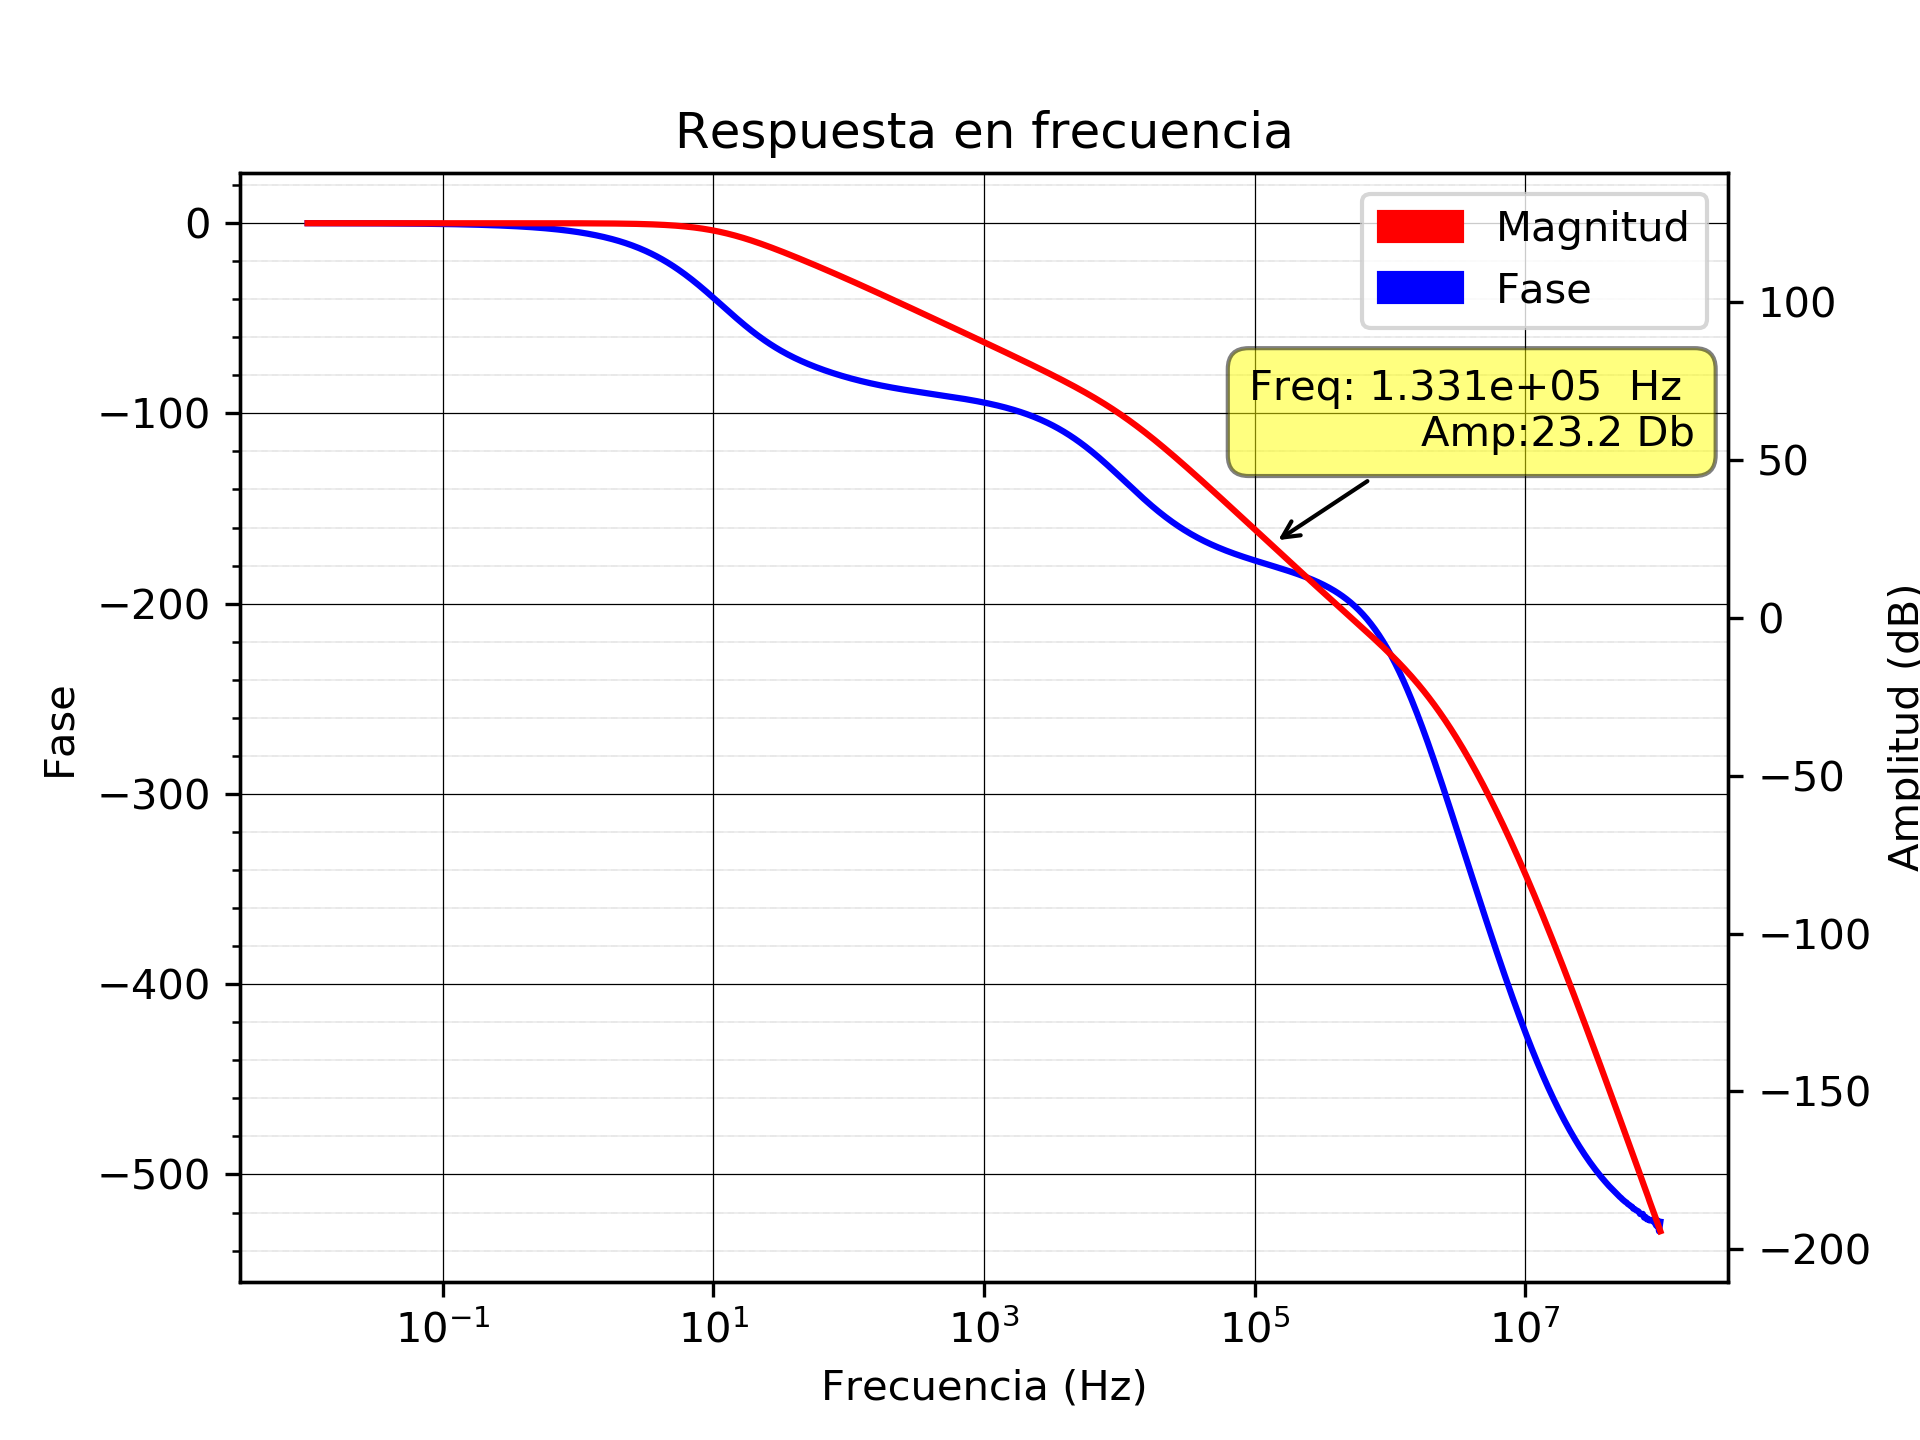
\includegraphics[scale=0.58]{Imagenes/Fuente_SinComp.png}
\par\end{centering}
\caption{Respuesta en frecuencia de la ganancia de lazo sin compensar}

\end{figure}

Como se indica en la respuesta obtenida, para cuando la fase cruza los $-180^{\circ}$ la ganacia es de $21dB$, que est\'a por encima de los $0dB$. Por lo tanto, hay altas probabilidades de que el circuito oscile sin carga. Como la oscilaci\'on ocurre a alta frecuencia, se observar\'ia la oscilaci\'on montada sobre la tensi\'on $V_O$ en DC esperada (seg\'un el valor del potenci\'ometro $R_4$). Con un volt\'imetro, no es posible observar esto dado que el valor medido es el valor medio, que ser\'ia la $V_O$ en DC esperada.

Para compensar esto, se coloc\'o un capacitor de $1uF$ entre la entrada no inversora del operacional y el colector del transistor $T_1$ del amplificador de error, m\'as un capacitor de $10uF$ a la salida del circuito (es decir en $V_O$), simulando en LTSpice para verificar que se realice la compensaci\'on.

\begin{figure}[!ht]
\begin{centering}
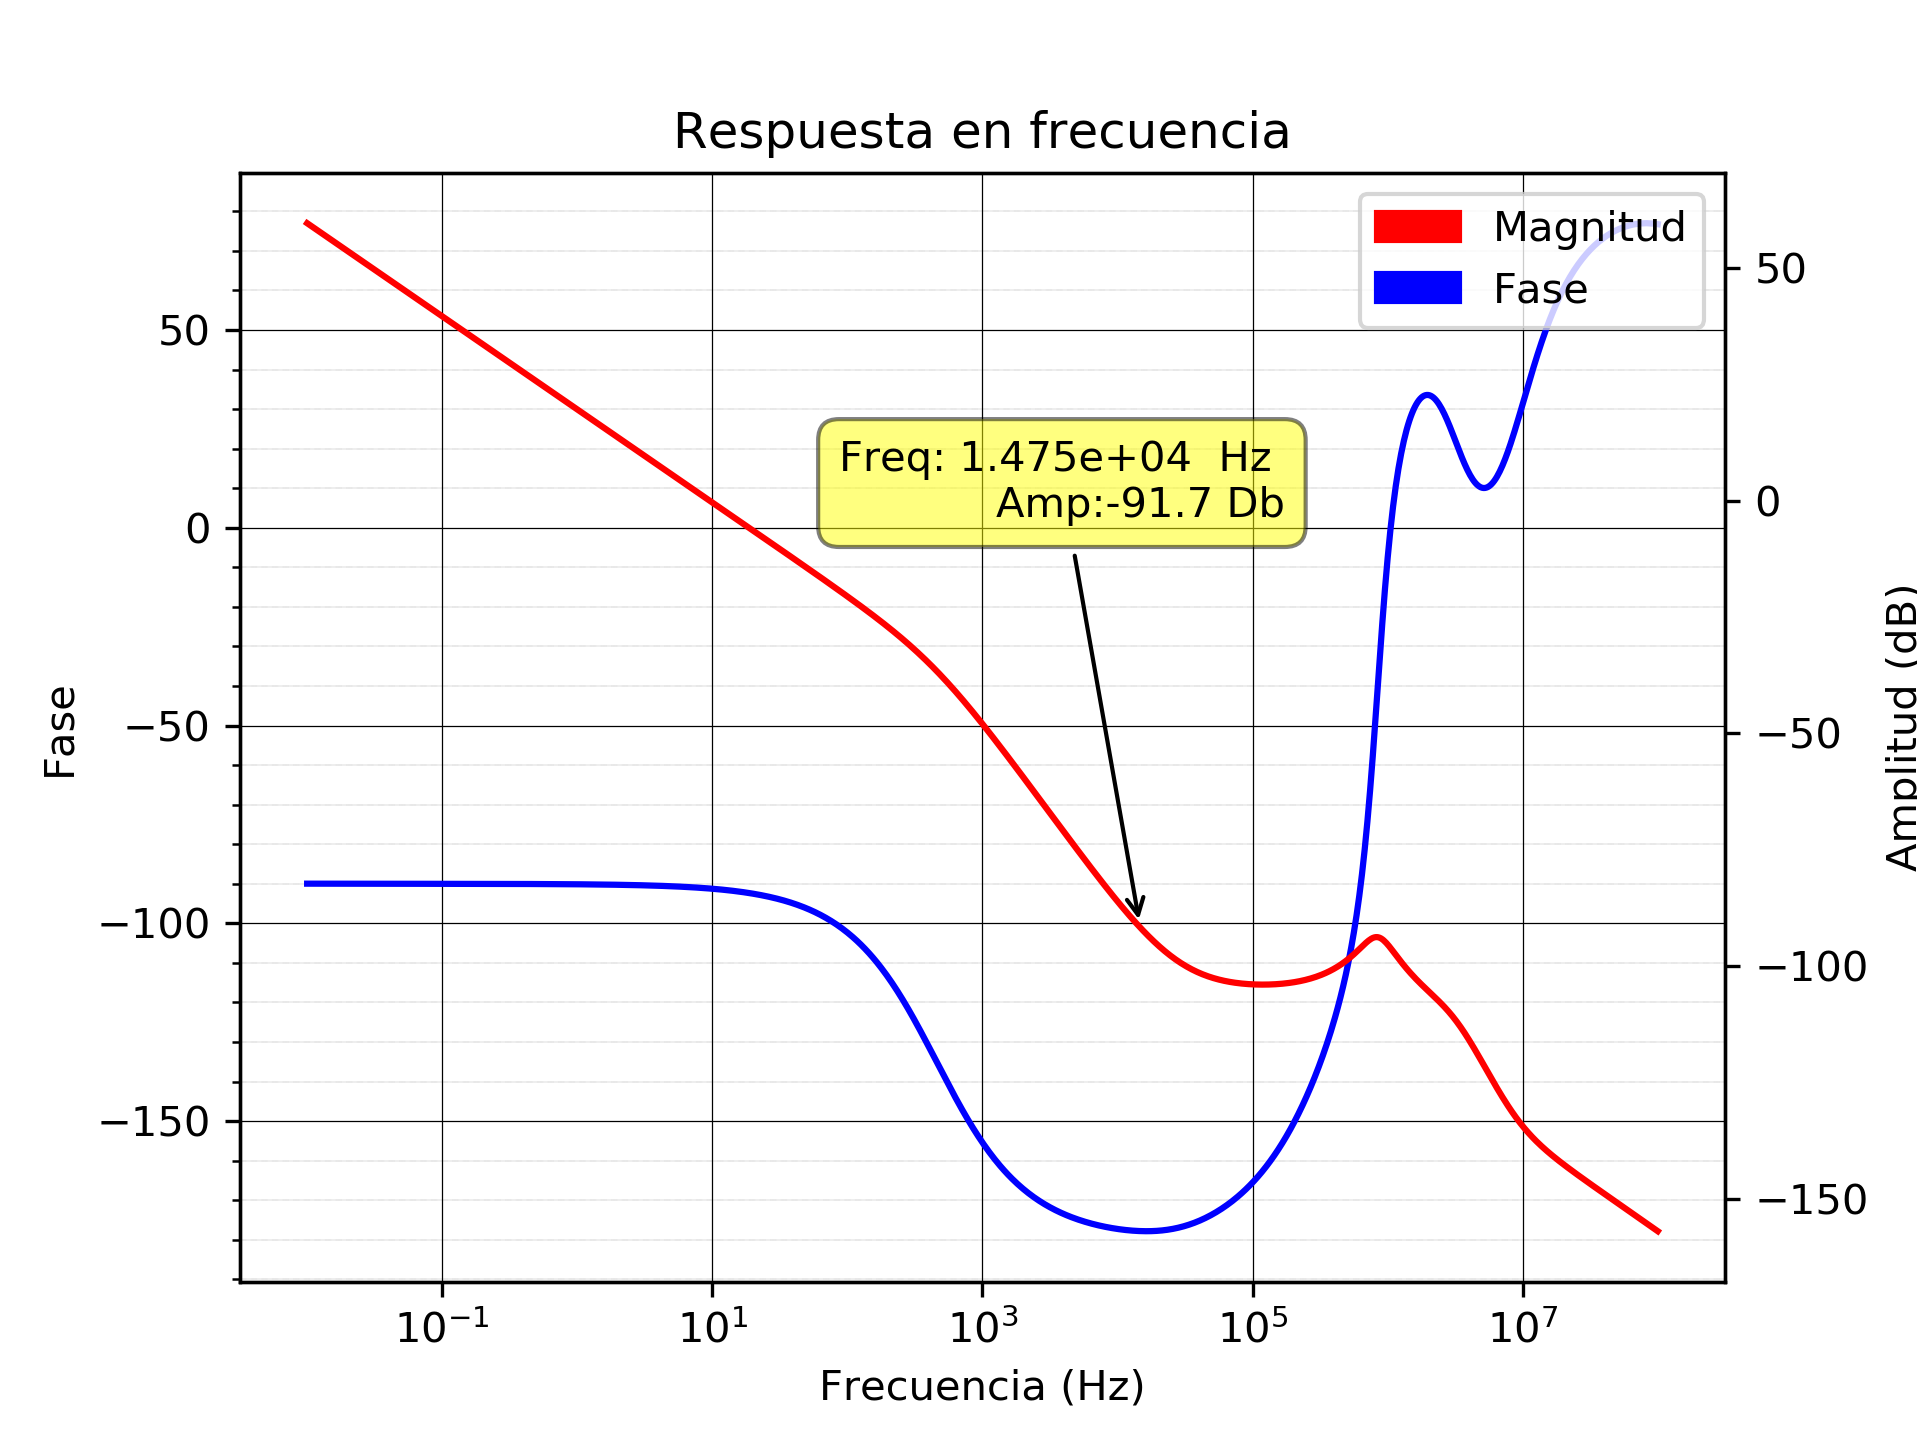
\includegraphics[scale=0.58]{Imagenes/Fuente_ConComp.png}
\par\end{centering}
\caption{Respuesta en frecuencia de la ganancia de lazo compensada}

\end{figure}

La respuesta en frecuencia resultante efectivamente logra cumplir con el objetivo de tener un margen de fase y de amplitud apropiados, disminuyendo la probabilidad de tener oscilaciones en la implementaci\'on real.

\newpage

\section{Implementaci\'on - Resultados}

\subsection{Caracter\'istica $V_O(I_O)$}

Utilizando el banco de pruebas, se registraron pares de valores $V_O$ - $I_O$ para trazar la curva caracter\'istica $V_O(I_O)$. Los valores tomados se muestran en la siguiente tabla.

\begin{table}[!ht]
\begin{centering}

\begin{tabular}[H]{|c|c|c|}
\hline 
RL & VO & IO\tabularnewline
\hline 
\hline 
$\infty$ & $10.09V$ & $0A$\tabularnewline
\hline 
$28.3 \Omega$ & $10V$ & $0.37A$\tabularnewline
\hline 
$13.6 \Omega$ & $9.95V$ & $0.77A$\tabularnewline
\hline 
$8.5 \Omega$ & $9.7V$ & $1.21A$\tabularnewline
\hline 
$6.5 \Omega$ & $9.56V$ & $1.55A$\tabularnewline
\hline 
$5.3 \Omega$ & $5.63V$ & $1.2A$\tabularnewline
\hline 
$3.9 \Omega$ & $3.24V$ & $1A$\tabularnewline
\hline 
$0 \Omega (CC)$ & $0V$ & $0.76A$\tabularnewline
\hline 
\end{tabular}
\par\end{centering}
\caption{Valores de $V_O(I_O)$ experimentales}

\end{table}

Con dichos valores, se compara ahora la caracter\'istica obtenida experimentalmente con la te\'orica y la simulada.

\begin{figure}[!ht]
\begin{centering}
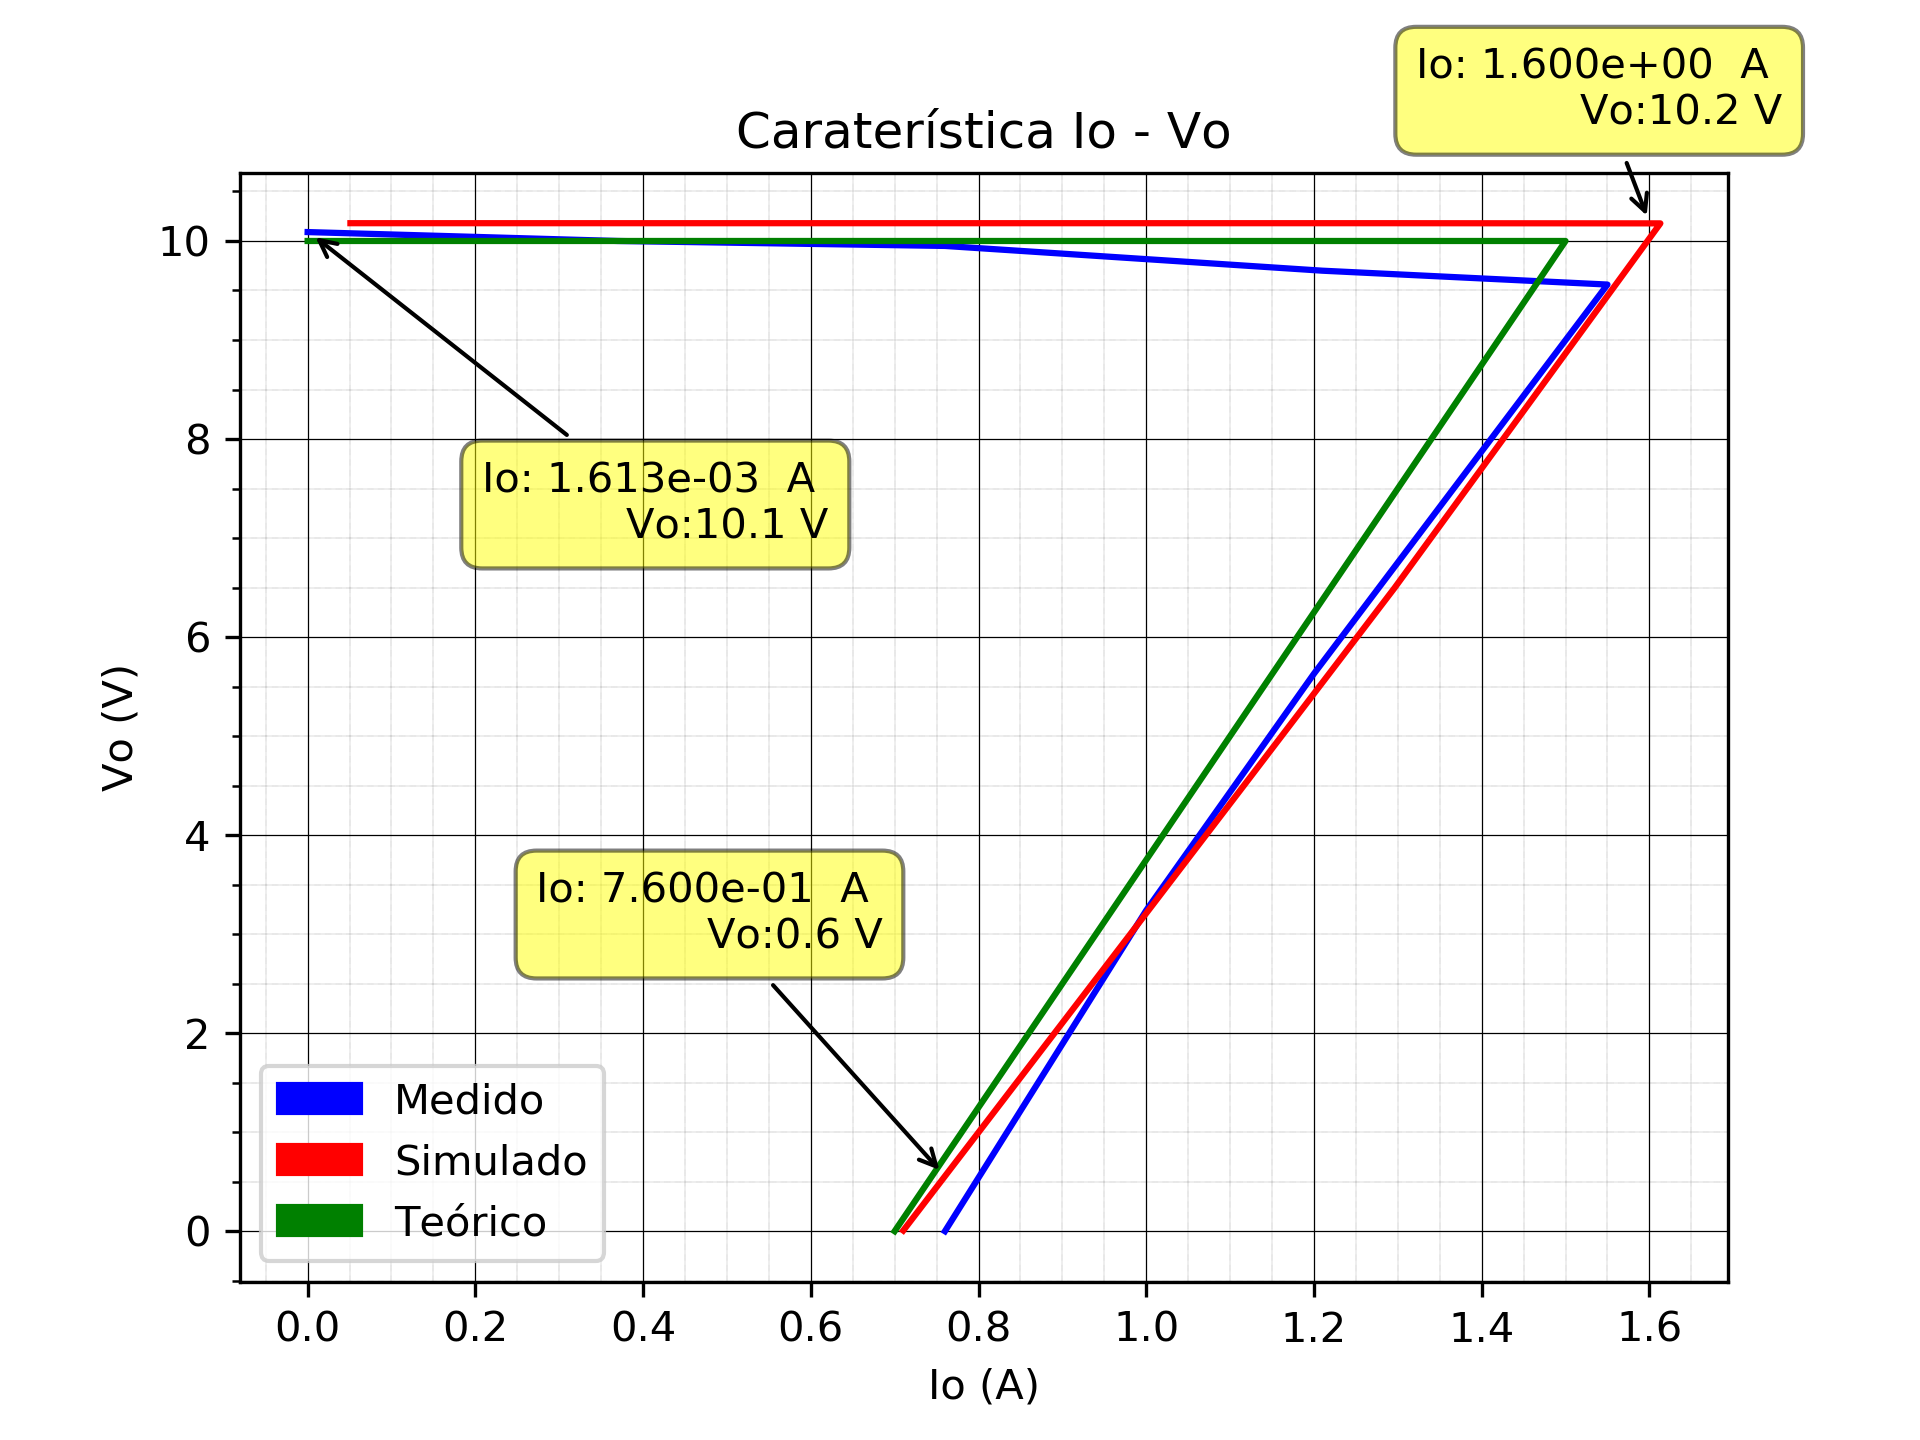
\includegraphics[scale=0.7]{Imagenes/Caracteristica_iovo.png}
\par\end{centering}
\caption{Caracter\'isticas de salida comparadas}

\end{figure}  

\subsection{Rendimiento}

Definimos el rendimiento de la fuente como la relaci\'on entre la m\'axima tensi\'on de salida $V_O$ y la m\'inima tensi\'on de entrada $V_R$, en porcentaje. Es decir:
\[
\eta \% = \frac{V_O}{V_R} \cdot 100
\]
Se calcula entonces el rendimiento con los valores de $V_O$ e $I_O$ te\'oricos, simulados y experimentales a carga m\'inima en regulaci\'on.
Se considera como valor de $V_O$ te\'orico m\'aximo $10.2V$ (es decir, incluyendo el margen), teniendo entonces:

\[
V_{R_{MIN}} = V_{O_{MAX}} + R_A \cdot I_{O_{MAX}} + V_{BE2_{ON}} + V_{CE3_{SAT}} + V_{R_1}
\]
\[
V_{R_{MIN}} =  = 10.2V + 1.6V + 1.4V + 0.7V + 0.7V = 14.8V 
\]

El valor de $V_O$ simulado fue de $10.18V$ con una $V_{R_{MIN}}= 14V$.

\begin{table}[!ht]
\begin{center}
\begin{tabular}{|c||c|c|c|}
\hline
& Te\'orico & Simulado & Experimental\\
\hline 
$\eta \%$ & 68\% & 72.7\% & 67.3\%\\
\hline 
\end{tabular}
\end{center}

\caption{Valores de rendimiento obtenidos}
\end{table}

\subsection{Impedancia de salida - $Z_O$}
 
Si la impedancia de salida fuera 0, en el caso de carga $R_{L_{MIN}}$ la $V_O$ deber\'ia ser la misma que para $R_L = \infty $. Como dicha impedancia no es nula, se puede medir un $\Delta V_O$ entre ambos casos de carga. De esta forma, se puede estimar un valor para la $Z_O$ (que ser\'a peque\~no) mediante:
\[
Z_O \simeq \frac{\Delta V_O}{I_{O_{MAX}}}   
\]
La caracter\'istica de tensi\'on real en general puede modelarse como se muestra a continuaci\'on.

\begin{figure}[!ht]
\begin{centering}
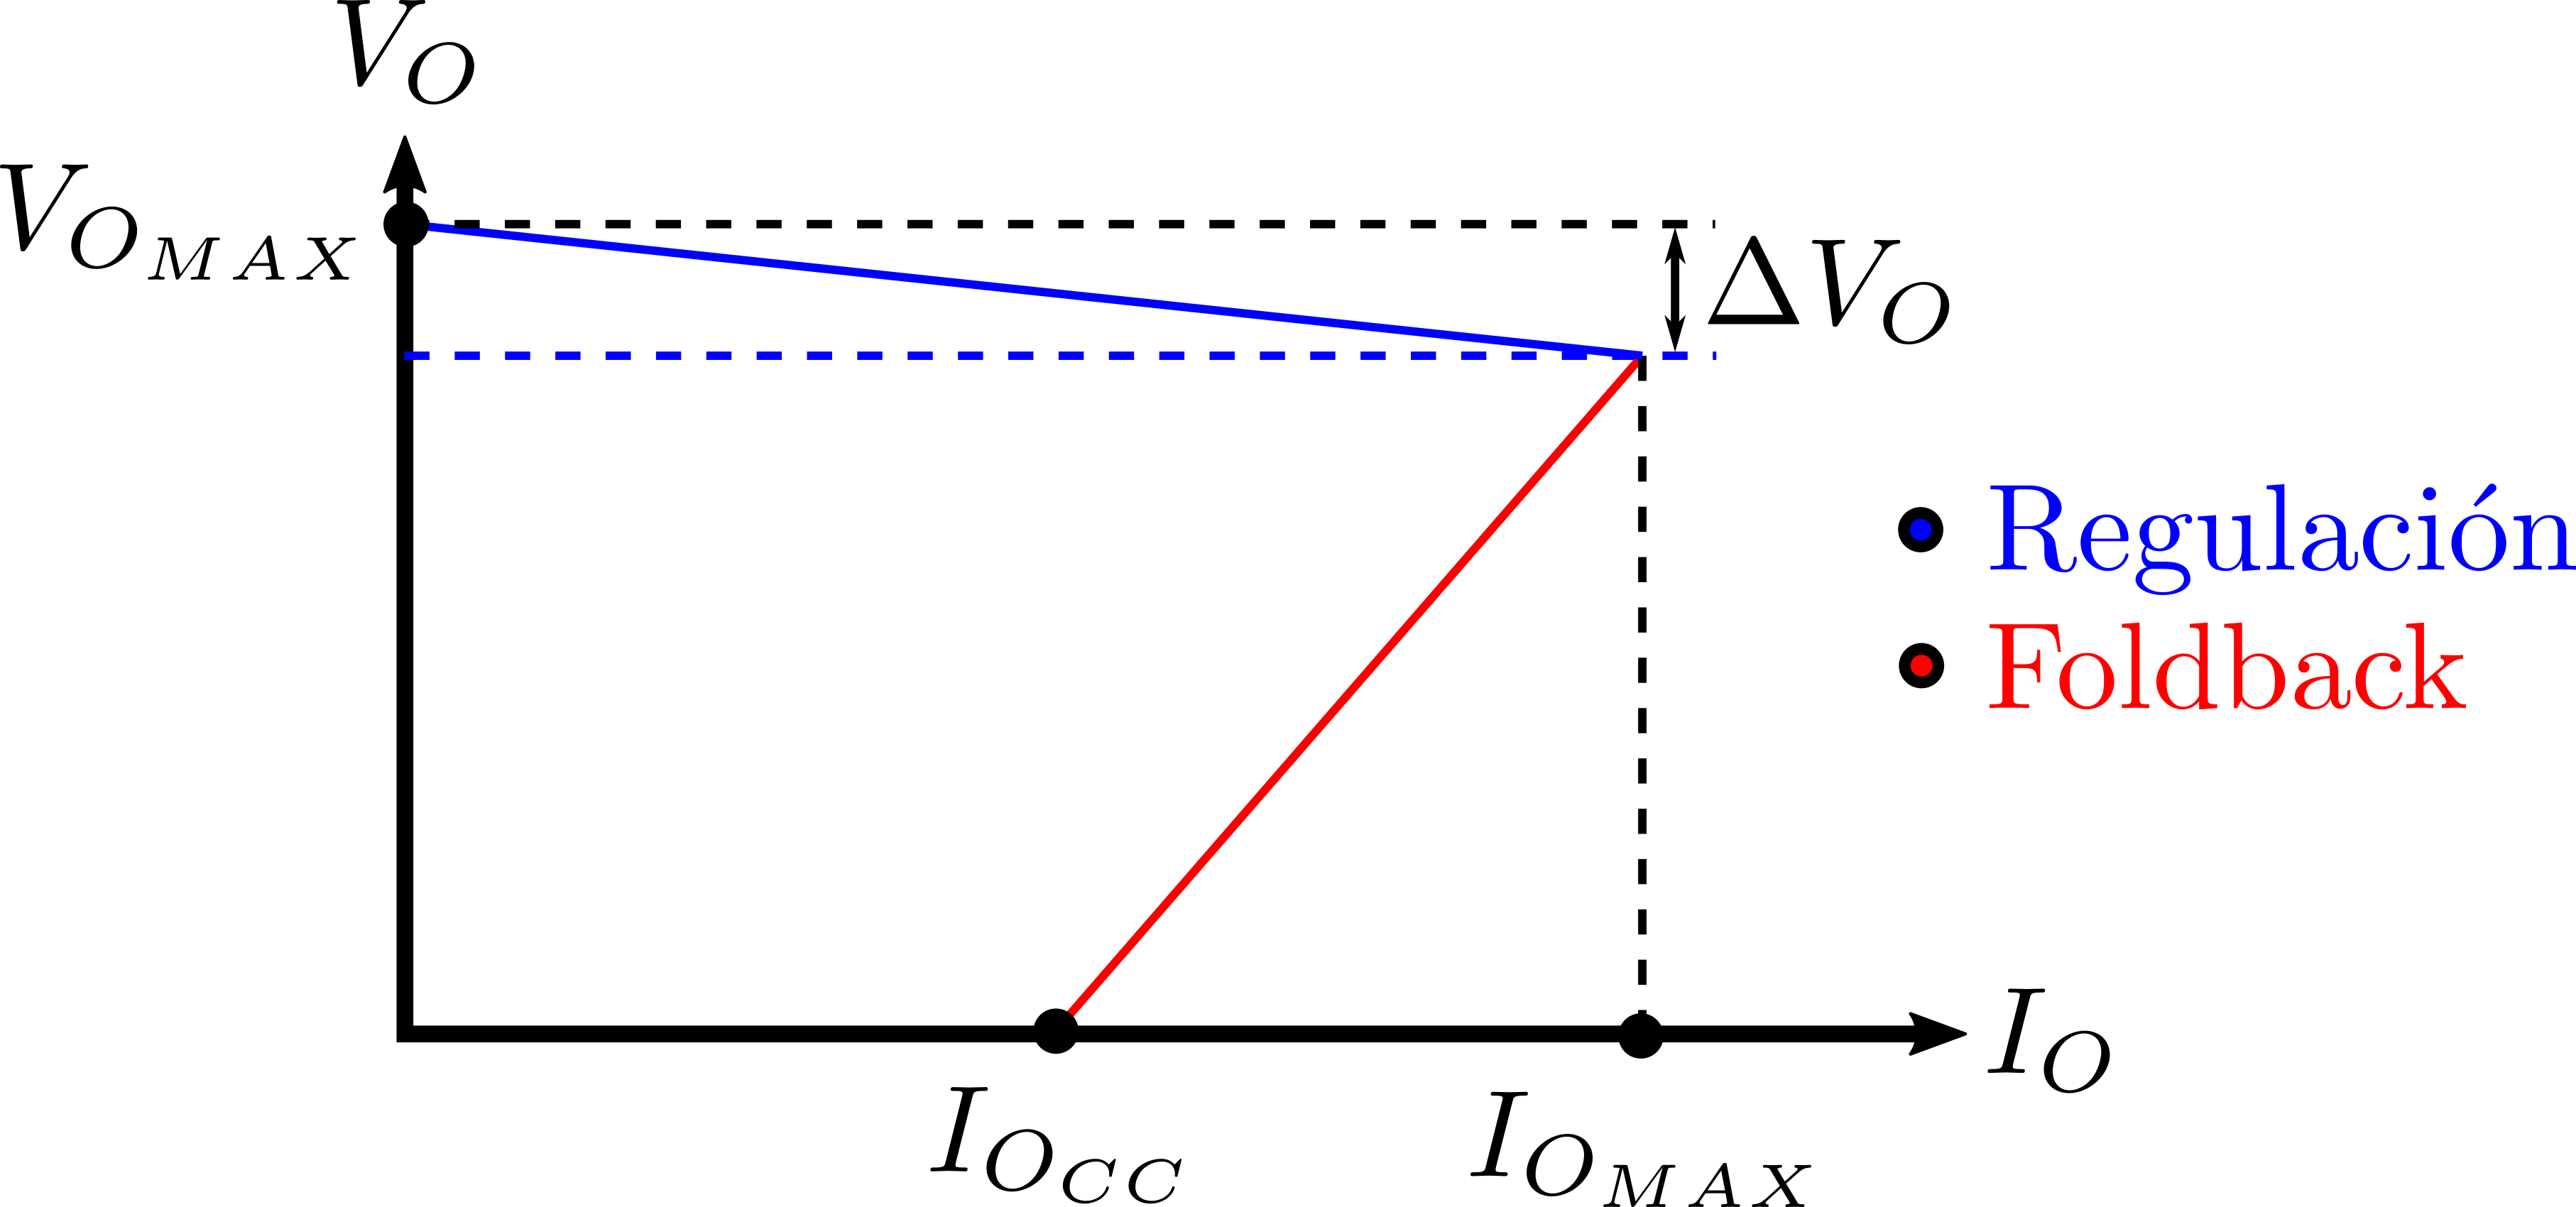
\includegraphics[scale=0.5]{Imagenes/FB_Real.png}
\par\end{centering}
\caption{Caracter\'istica de salida real con protecci\'on Foldback}

\end{figure}

En el caso experimental, como dicha pendiente puede cambiar en el trayecto desde $0A$ hasta $I_{O_{MAX}}$, se tomo de referencia el caso con carga $R_L = \infty$ y un caso intermedio, donde pudiera medirse m\'as claramente una $V_O$ diferente al primer caso, para obtener un estimador de $Z_O$. Dichos valores tomados se indican en el siguiente cuadro, obteniendo un estimador de $Z_O$ experimental comparado con el te\'orico y el simulado.


\begin{table}[!ht]

\begin{center}
\begin{tabular}{|c||c|c|c|}
\hline
& Te\'orico & Simulado & Experimental\\
\hline 
$\Delta V_O$ & $0V$ & $2mV$ & $10.09V-9.95V=0.14V$\\
\hline 
$I_O$ &  $1.5A$    &   $1.61A$     & $0.77A - 0A = 0.77A$\\
\hline
$Z_O$ &   $0\Omega$   &    $1.2m\Omega$    & $0.2\Omega$\\
\hline
\end{tabular}
\end{center}

\caption{Valores de $Z_O$ obtenidos}
\end{table}


\subsection{PSRR - Power Supply Rejection Ratio}

La relaci\'on de rechazo del ripple de la entrada en la salida se la define como:

\[
PSRR = 20 \cdot log \left( \frac{\Delta V_R}{\Delta V_O} \right)
\]

Para la simulaci\'on y la experimental, se toma el $\Delta V_O$ para carga m\'inima y sin carga, obteniendo los siguientes resultados.

\begin{table}[!ht]
\centering
\begin{tabular}{|c|c|c|c|}
\hline
\multicolumn{2}{|c|}{}                         & Simulado & Experimental \\ \hline
\multirow{3}{*}{$R_L = \infty$} & $\Delta V_R$ &  $2V$    & $213mV$              \\ \cline{2-4} 
                                & $\Delta V_O$ &  $0.013V$& $80mV$             \\ \cline{2-4} 
                                & PSRR         &  44dB    & 8.5dB              \\ \hline
\multirow{3}{*}{$R_{L_{MIN}}$}  & $\Delta V_R$ &  $2V$    &  $3.19V$            \\ \cline{2-4} 
                                & $\Delta V_O$ &  $0.04V$ & $1.69V$              \\ \cline{2-4} 
                                & PSRR         &  34dB    &  5.52dB            \\ \hline
\end{tabular}
\caption{Valores de PSRR}

\end{table}

En el caso de la simulaci\'on da un valor m\'as grande dado que la fuente utilizada es una senoidal que var\'ia $15V$ y $17V$ ideal, es decir que no cae su valor al disminuir la carga $R_L$, por lo que el valor obtenido es m\'as preciso.
En el caso experimental, se utiliz\'o una fuente de $15V$ de DC con ripple, pero cuyo valor nominal disminuye al cargarla y exigirle corrientes altas, lo que modifica los puntos de polarizaci\'on en forma considerable.
En cualquier caso, tanto el simulado como el medido coinciden en que el PSRR empeora al exigir corriente.

\newpage

\section{Dise\~no de PCB - Consideraciones}

Al momento de realizar la implementaci\'on en PCB, como es una placa de potencia, se tienen en cuenta ciertas cuestiones en relaci\'on al ruteo y espacio de componentes.

\subsection{Placa fuente}

Para implementar la fuente, teniendo en cuenta los requerimientos de espacio y potencia:

\begin{itemize}
\item Dado que el transistor lleva un disipador, se lo coloc\'o cerca de uno de los bordes, de manera tal que el disipador quede hacia afuera.
\item Para la alimentaci\'on y salida, se utilizaron conectores polarizados,
\item Se incluyeron soportes tipo tameco en las esquinas para mantener el PCB en pie.
\end{itemize}

\begin{figure}[!ht]
\begin{centering}
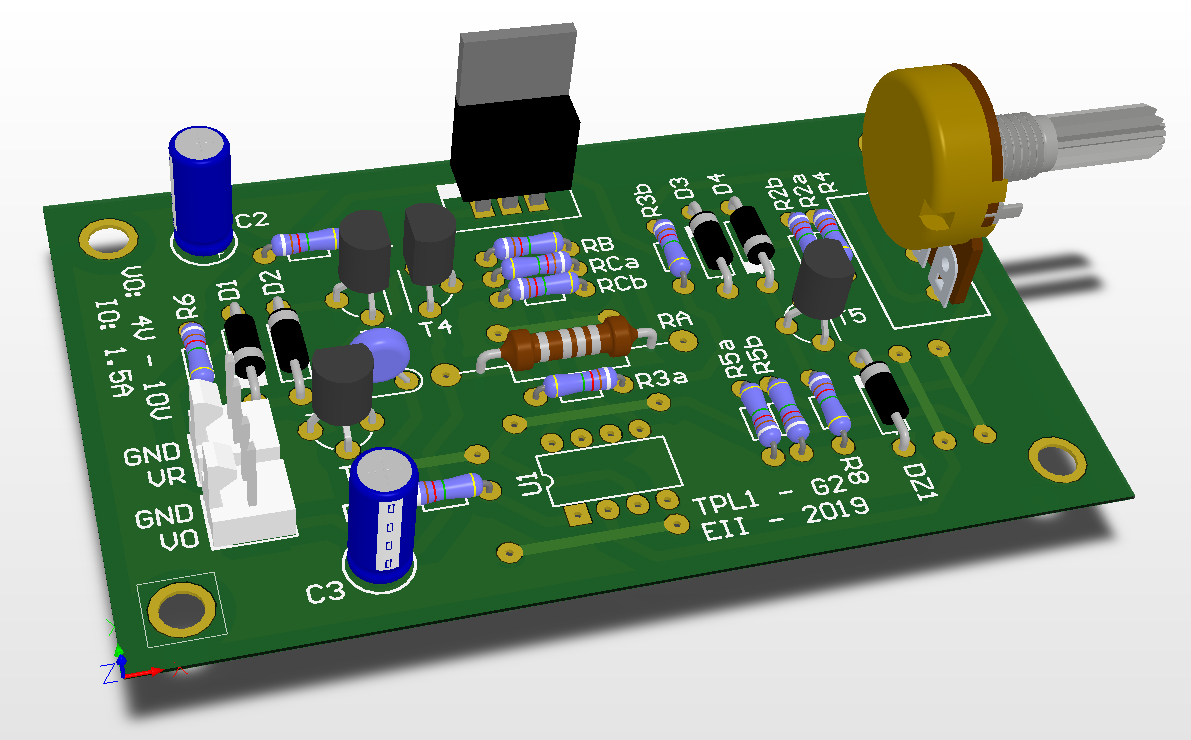
\includegraphics[scale=0.45]{Imagenes/Fuente3D.png}
\par\end{centering}
\caption{Modelo 3D del PCB de la fuente}

\end{figure}

\subsection{Placa de banco de pruebas}

Para poder realizar mediciones con carga $R_L$ sobre la curva de foldback, se implement\'o una placa como banco de pruebas con resistencias de potencia de $15\Omega$, $10\Omega$, $1\Omega$ y $0.47\Omega$. De esta manera se logra tener cargas resistivas puras, evitando utilizar un re\'ostato debido a la gran inductancia que posee.

\begin{figure}[!ht]
\begin{centering}
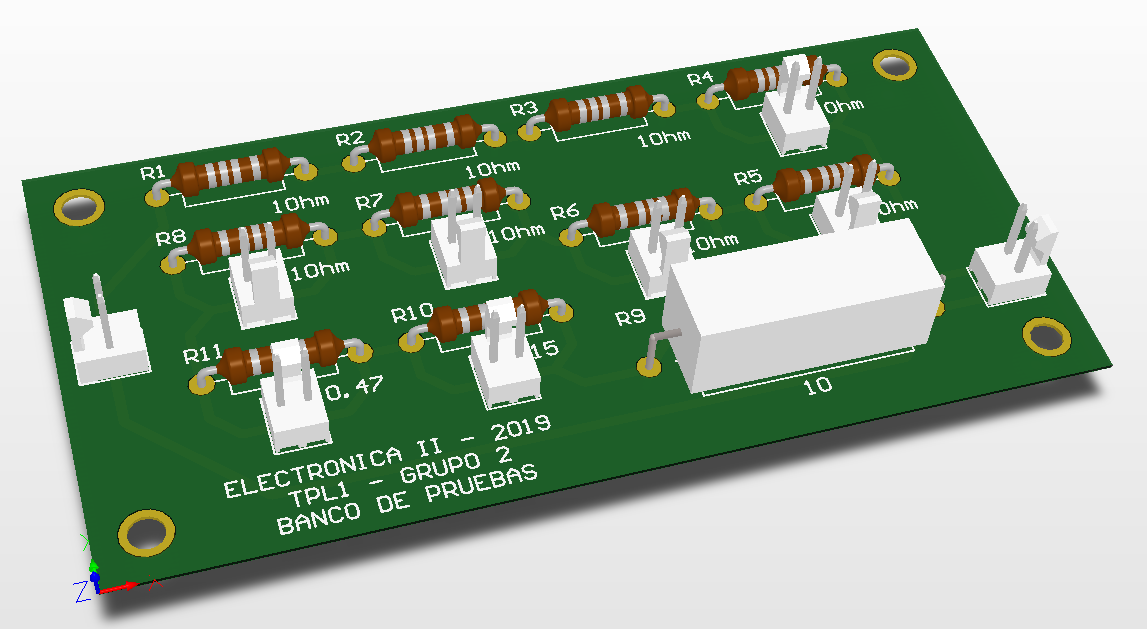
\includegraphics[scale=0.45]{Imagenes/Banco3D.png}
\par\end{centering}
\caption{Modelo 3D del PCB del banco de pruebas}

\end{figure}

\end{document}